\documentclass[12pt]{article}
\usepackage{geometry}
 \geometry{
 a4paper,
 total={170mm,257mm},
 left=20mm,
 top=20mm,
 }
\usepackage[skip=5pt plus1pt, indent=25pt]{parskip}
\usepackage{graphicx} % Required for inserting images
\usepackage[utf8]{inputenc} % allow utf-8 input
\usepackage[T1]{fontenc}    % use 8-bit T1 fonts
%\usepackage{hyperref}       % hyperlinks 
\usepackage{url}            % simple URL typesetting
\usepackage{booktabs}       % professional-quality tables
\usepackage{amsfonts}       % blackboard math symbols
\usepackage{nicefrac}       % compact symbols for 1/2, etc.
\usepackage{microtype}      % microtypography
\usepackage{amsmath}
\usepackage{amssymb}
\usepackage{dsfont}
\usepackage{bm}
%\usepackage{xcolor}         
\usepackage[spanish]{babel}
\usepackage[table,xcdraw]{xcolor} % colors
\usepackage{gensymb}
\usepackage{caption}
\usepackage{subcaption}
\usepackage{svg}
\usepackage{multirow}
\usepackage{dirtree}
\graphicspath{{Images/}}
\svgpath{{Images/}}

\title{Trabajo de especialización}
\author{
    Federico Checozzi \\
    \textrm{tiamantex@hotmail.com} 
    }
\date{}
%\renewcommand*\contentsname{}

\begin{document}
\maketitle

\begin{abstract}
En este trabajo se entrenan y comparan clasificadores basados en métodos clásicos de aprendizaje estadístico para aplicaciones de quimiometría (LDA, QDA y PCA) y técnicas modernas de aprendizaje automático (LightGBM, UMAP y SOM), para diferenciar espectros de emisión de cuatro tipos de suelo diferentes obtenidos por espectroscopía de plasma inducido por láser (LIBS), con el auxilio de distintas técnicas de reducción dimensional.

Adicionalmente se investiga el uso del análisis de componentes principales robusto y tests de hipótesis para estudiar la estructura de los datos, así como también se hace un análisis estadístico y gráfico del funcionamiento y problemas de estabilidad numérica de los diferentes algoritmos utilizados.

Se concluye que los tipos de suelo son separables mediante modelos con fronteras de decisión lineales y que el uso de modelos y transformaciones más complejos son contraproductivos para esta aplicación porque intercambian sesgo, el cual genera errores mínimos en un modelo simple, por varianza. Esto no necesariamente se extiende a conjuntos de datos de estructura más compleja.
\end{abstract}

\tableofcontents
\newpage
\section{Introducción}
\subsection{Espectroscopía de plasma inducida por láser}

La espectroscopía es la ciencia que se concierne con la investigación y medición de espectros producidos cuando materiales interactúan o emiten radiación electromagnética\cite{Spectroscopy}. En particular, en la espectroscopía de plasma inducida por láser (LIBS) un rayo láser enfocado es usado para generar vapor de plasma en la superficie de muestras líquidas y sólidas, o dentro del volumen de una muestra de gases, líquidos y aerosoles. Cada átomo excitado en el plasma emite un único conjunto de líneas espectrales, particularmente en la región óptica del espectro. Esta emisión óptica puede ser recolectada y analizada para determinar la composición química de una muestra. El plasma puede ser generado usando un único pulso láser o usando pulsos de forma repetitiva. Esta técnica permite un análisis remoto de muestras debido a que solo los fotones del láser deben entrar en contacto con la muestra.

Esta técnica tiene una ventaja distintiva sobre otras ya que requiere poca o ninguna preparación de la muestra antes del análisis y puede ser usada para un análisis rápido en tiempo real. Tampoco hay requerimientos específicos de que la muestra sea fluorescente como en las espectroscopías Raman o infrarroja.

\subsubsection{Principios básicos}

LIBS es una técnica simple de implementar en la práctica. Un rayo láser de alta potencia (pulsos con un período del orden de nanosegundos con una longitud de onda en el orden de micrometros) son enfocados a través de una lente para producir un plasma. La luz emitida es recolectada, frecuentemente a través de una fibra óptica, y dirigida a un espectrometro\cite{LIBS}. Un diagrama esquemático de un banco típico puede verse en la Figura \ref{fig:LIBS1}.

\begin{figure}[htbp]
    \centering
    %\captionsetup{justification=centering}
    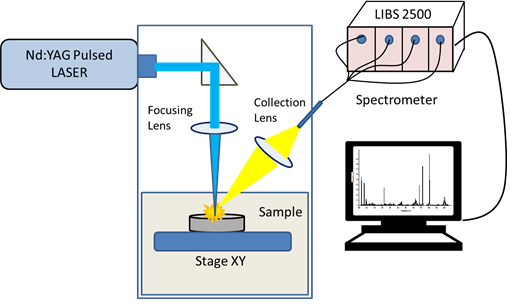
\includegraphics[width=15cm]{Esquema LIBS.png}
    \caption{\textbf{Esquema típico de un experimento LIBS.} 1) Láser pulsado 2) Muestra 3) Fibra óptica  4) Espectrómetro 5) Programa de adquisición.}
    \label{fig:LIBS1}
\end{figure}

Hay dos procesos principales que pueden iniciar la ionización de especies moleculares y atómicas\cite{LIBS}: ionización directa de la muestra por ionización multifotónica y el proceso de absorción bremsstrahlung inverso. 

En el primero, los átomos o moléculas absorben simultáneamente un número suficiente de fotones para causar la ionización (o eyección de electrones de la banda de valencia a la de conducción, en el caso de metales). Esta emisión solo es significativa para longitudes de onda menores que $1 \mu m$ y intensidades mayores que $10^{10}\frac{W}{{cm}^2}$. Longitudes de onda mayores hacen que sea poco probable que se absorban suficientes fotones para incrementar la energía encima del potencial de ionización. Este proceso es importante también a bajas presiones donde pocas colisiones ocurren debido a la baja densidad de partícula del medio.

El segundo involucra la absorción de un fotón por uno o más electrones semilla (generados por radiación natural o los primeros fotones de un pulso láser al colisionar con partículas en el entorno) presentes en el volumen focal al comienzo del pulso láser. Los electrones adquieren energía de la absorbancia de fotones y por colisiones con átomos, iones y moléculas. Si la energía de un electrón libre es mayor que el potencial de ionización de una especie neutral, puede ionizarla al colisionar. Esto resulta en dos electrones libres, los cuales pueden ganar más energía a partir del campo eléctrico causando la ionización de otros neutrales. Con el incremento de la población de iones y electrones en el volumen focal, la probabilidad de colisiones entre electrones y fotones aumenta, resultado en una multiplicación de electrón y crecimiento en cascada. Este proceso es tan dramático que todas las especies vaporizadas de la superficie del sustrato pueden ser ionizadas causando un incremento en el crecimiento del plasma y el acoplamiento del láser dentro del plasma. Esto resulta en un plasma ópticamente opaco que proteje al sustrato del resto del pulso láser. Este proceso será dominante en altas presiones (donde los efectos colisionales son fuertes) o para longitudes de onda mayores que $1 \mu m$.

Durante el tiempo de vida del plasma, el espectro de emisión cambia como una función del tiempo. En la fase más temprana, hay una fuerte componente de luz blanca (principalmente bremsstrahlung y radiación de recombinación), la cual contiene poca información útil para espectroscopía. Tras el pulso láser, el continuo gradualmente desaparece permitiendo que sean detectadas señales espectroscópicas débiles de los elementos de interés. Esto suele ocurrir en un tiempo mayor que la duración del pulso. La medición se hace en una ventana de tiempo tras el pulso, la cual no debe ser demasiado grande para evitar captar la luz ambiental.

\subsubsection{Mejoras de calidad y reproducibilidad de las mediciones}
Pueden realizarse varias optimizaciones con el objetivo de mejorar la calidad de los ensayos experimentales realizados mediante LIBS\cite{LIBS}:

\begin{itemize}
    \item Una forma de mejorar la señal de emisión es realizar mediciones en vacío para evitar el espectro emitido por el aire alrededor de la muestra, o alternativamente el uso de un gas inerte para desplazar el aire y mejorar la calidad del plasma. Para este último, el uso de argón será preferible al helio, debido a que el argón es un gas más pesado y por lo tanto menos eficiente para enfriar la muestra (lo cual implica una mayor temperatura de plasma y mayor densidad de electrones).

    \item También suele utilizarse pulsos dobles para producir mejoras de seña. Típicamente, LIBS tiene límites de detección en el rango de ppm. El uso de esta estrategia permite superar esta deficiencia. Dado que la mayoría de la energía del láser es absorbida por la muestra y el vapor generado, impactos sucesivos pueden ser utilizados para recalentar el plasma que contiene las especies ionizadas, causando un incremento significativo en la emisión de las especies encontradas en el vapor.

    \item Por último, el uso de pulsos cortos y radiación ultravioleta mejoran la reproducibilidad de este método al reducir el efecto de transferencias de calor por toda la muestra, reducir efectos de derretimiento y aumentar la eficiencia con la que se desintegra la muestra debido a que los fotones son más energéticos con ese tipo de radiación.
\end{itemize}

\subsection{Quimiometría}

La quimiometría es una disciplina química que usa métodos estadísticos y matemáticos, para designar o seleccionar procedimientos y experimentos óptimos, y proveer la mayor cantidad de información química posible analizando datos químicos\cite{Chemo}. La parte más importante de esto es la aplicación de análisis de datos multivariados a datos relevantes químicamente. 

Los sistemas químicos y físicos de interés práctico son a menudo demasiado complicados y no pueden ser descriptos suficientemente por la teoría, por lo cual una aplicación típica de quimiometría no está basada en primeros principios sino que está enfocada en el análisis de datos. El análisis multivariado es una herramienta poderosa para analizar y estructurar cojuntos de datos que hayan sido obtenidos de estos sistemas, y para crear modelos matemáticos empíricos que son capaces de predecir los valores de propiedades importantes que no son directamente medibles. Estas técnicas consideran muchas variables en conjunto y mejoran la capacidad de evaluación de datos.

\subsubsection{Enfoques estadístico y de aprendizaje automático}

Hay dos enfoques posibles en el análisis de datos multivariado: Uno está impulsado por los datos, y las herramientas estadísticas son vistas como algoritmos que son aplicados a la obtención de resultados; el otro se basa en el uso de modelos en los que los datos son asumidos como el resultado de procesos aleatorios. Los tipos de datos en quimiometría requieren un enfoque mayormente basado en datos: las suposiciones de distribución no se cumplen, el número de variables es más alto que el número de objetos, las variables están altamente correlacionadas\cite{Chemo}. Aún así, el tratamiento estadístico de los diferentes algoritmos utilizados llevó a mejoras como la robustificación. Por lo tanto, ambos enfoques tienen su propio derecho a existir y una combinación de ambos puede ser una gran ventaja.

%citar artículo de enciclopedia
Algunas de las técnicas tradicionales de aprendizaje automático (pero con un origen en el mundo estadístico) así como ciertas técnicas aplicadas específicamente a espectroscopía son\cite{STATS}\cite{F-ENG}:

\begin{itemize}
    \item \textbf{Ingeniería de atributos:} Centrado por media, doble centrado, variado normal estándar (SNV), corrección por dispersión multiplicativa (MSC), suavizado por primera y segunda derivada, filtro de media, mediana y Savitzky-Golay, derivación, integración de regiones con picos, intensidad en picos, e índices de la habilidad del equipo para separar espectros, submuestreo de longitudes de onda, entre otros. 
    \item \textbf{Reducción de la dimensionalidad:} El análisis de componentes principales (PCA) es una de las técnicas más comunmente utilizadas. También tiene usos exploratorios.
    \item \textbf{Clustering:}  El análisis por clustering jerárquico (HCA) y K-medias son los métodos más populares.
    \item \textbf{Calibración:} la predicción de respuestas cuantitativas continuas como la concentración de analitos. La regresión por componentes principales (PCR) y la regresión de mínimos cuadrados parciales (PLS) son los métodos más utilizados. La segunda técnica en particular surgió en el mundo de las ciencias sociales pero se popularizó gracias a aplicaciones de quimiometría.
    \item \textbf{Clasificación:} son utilizadas la regresión logística, el análisis discriminante lineal (LDA) y cuadrático (QDA) de Fisher (estos son aún caballos de bastalla para métodos paramétricos), el análisis discriminante regularizado (RDA) y el análisis discriminante por mínimos cuadrados parciales (PLS-DA).
\end{itemize}

%citar review y bastante de lo de abajo
Como alternativa a estas, hay técnicas modernas más intensivas computacionalmente en general propias del mundo del aprendizaje automático, como por ejemplo\cite{ML}\cite{GA}\cite{PCA-SVM}\cite{MULT}\cite{CLUST}\cite{SOM}\cite{EMSLIBS2019}:

%https://journals.plos.org/plosone/article?id=10.1371/journal.pone.0266369    clustering
%https://journals.sagepub.com/doi/10.1255/jnirs.778  algoritmos genéticos
\begin{itemize}
    \item \textbf{Ingeniería de atributos:} son usados la selección de variables por métodos típicos (selección hacia adelante, hacia atrás y bidireccional), algoritmos genéticos (GA) y la importancia de variables extraídas de ensembles de árboles, entre muchísimos otros.
    \item \textbf{Reducción de la dimensionalidad:} son utilizados autoencoders, varias técnicas de aprendizaje de variedad: mapeo isométrico (ISOMAP), escalamiento multidimensional (MDS), \textit{t-distributed Stochastic Neighbor Embedding} (t-SNE), aproximación y proyección uniforme de variedad (UMAP), mapas autoorganizados (SOM) y muchos otros más.
    \item \textbf{Clustering:} son utilizados el particionado por medoides (PAM), clustering espacial basado en densidad de aplicaciones con ruido (DBSCAN), clustering espectral, clustering difuso, entre otros.
    \item \textbf{Calibración y clasificación:} son utilizadas la regresión y clasificación por redes neuronales (ANN), máquinas de vectores de soporte (SVM) y en menor medida ensembles de árboles (RF, XGBoost, LightGBM, etc.).
\end{itemize}

\subsubsection{Ejemplos de aplicación}

\begin{itemize}
    \item Ozturk et al. utilizan espectroscopía infrarroja para clasificar alimentos en polvo\cite{F-ENG}. Se experimenta con una amplia gama de técnicas de preprocesamiento (centrado, filtro de media, de Savitzky-Golay, suavizado por derivadas, autoencoders, etc.) en combinación con SVM y ANN.
    \item Lavine, Davidson y Moores utilizan GA para seleccionar longitudes de onda que maximizen la separación entre grupos en una aplicación de reconocimiento de patrones espectrales\cite{GA}. 
    \item Dahlstrand et al. utilizan espectroscopía infrarroja para diferenciar cinco tipos de tejido dérmico porcino\cite{PCA-SVM}. Se utiliza PCA y SVM para entrenar un clasificador con un 98\% de exactitud.
    \item Mwanga et al. utilizan espectroscopía infraroja para clasificar muestras de sangre vertebradas obtenidas en vectores de malaria\cite{MULT}. Se eliminan ciertas bandas espectrales de poco interés (agua, $CO_2$ y regiones planas), y se emplean KNN, LR, SVM, NB, RF, XGBoost y ANN. Se obtienen los mejores resultados con LR.
    \item Crase y Thennadil desarrollan una metodología de selección de algoritmos de clustering aplicado a espectroscopía\cite{CLUST}. Experimentan sobre diversos conjuntos de datos empleando MSC en la etapa de preprocesamiento, PCA y t-SNE para reducción dimensional, y HCA, PAM, DBSCAN, entre otros, para clustering.
    \item Shan et al. realizan calibraciones en base a dos conjuntos de datos infrarrojos: uno de fermentación de ácido $\gamma$-poliglutámico y otro de extracción de paeoniflorina\cite{SOM}. Se utiliza SOM, PLS y otras técnicas.
    \item De particular interés para este trabajo resulta la variedad de enfoques ilustrada por la competencia de clasificación del Décimo Simposio Euromediterráneo sobre LIBS (EMSLIBS 2019), para la clasificación de hematitas\cite{EMSLIBS2019}: PCA, LDA, submuestreo de variables, índices espectrales de habilidad de equipo, PLS-DA, autoencoders, UMAP, ANN e importancias de variables. Si bien son aplicaciones en un contexto de mayor complejidad, las técnicas presentadas fueron la fuente de ideas principales para este trabajo. Estas diferentes técnicas muestran la ventaja de un uso judicioso de ingeniería de atributos en combinación con técnicas quimiométricas tradicionales, aunque métodos modernos también fueron competitivos.
\end{itemize}

\section{Objetivos}

El presente trabajo busca entrenar y comparar clasificadores capaces de diferenciar entre espectros provenientes de muestras de suelo de cuatro tipos diferentes, empleando metodologías clásicas provenientes de la estadística (análisis de componentes principales y análisis discriminante ñineal) así como metodologías modernas provenientes del aprendizaje automático (LightGBM, y se usa de forma auxiliar varias técnicas de reducción dimensional como mapas autoorganizados, y aproximación y proyección uniforme de variedad).

Una meta adicional es una exploración detallada del conjunto de datos utilizado mediante el Análisis de Componentes Principales y tests de hipótesis de las propiedades de los datos, con el objetivo de entender las diferencias entre clases y longitudes de onda más relevantes, así como detectar espectros atípicos y caracterizarlos.

\section{Datos}

%la descripción de LIBS iría en la introducción
El conjunto de datos utilizado en este trabajo fue provisto por el International Centre for Earth Studies (ICES). Este mismo consiste de 156 archivos de valores separados por comas (CSV) correspondientes a espectros químicos extraídos de cuatro tipos diferentes de suelo obtenidas mediante LIBS extraído en terreno cercano a una mina en la cordillera de los Andes, originalmente con el propósito de medir niveles de contaminación. 

El equipamiento utilizado (ver Figura \ref{fig:LIBS2}) en las mediciones de los espectros consistió de un láser Q-Conmutado Nd:YAG (\textit{Quanta Ray INDI}) con una longitud de onda fundamental $\lambda = 1064nm$, una duración de pulso de $9ns$ y una longitud focal de $15cm$. En orden de obtener la máxima intensidad de señal, se estableció una energía óptima de $\frac{50mJ}{pulso}$ para la adquicisión de espectros con $1,67\mu s$ de tiempo de demora en orden de minimizar la señal de fondo. Esta demora es el tiempo tras el cual el láser vaporiza el material y el espectrómetro empieza la adquisición. Un espectrómetro Ocean Optics modelo \textit{LIBS 2500 plus} fue usado en el rango de $293,83nm$ a $729,06nm$. Cada muestra fue adquirida como el resultado de 20 láseres pulsados en diferentes puntos de la superficie de pastillas elaboradas a partir de las muestras de suelo.

\begin{figure}[htbp]
    \centering
    %\captionsetup{justification=centering}
    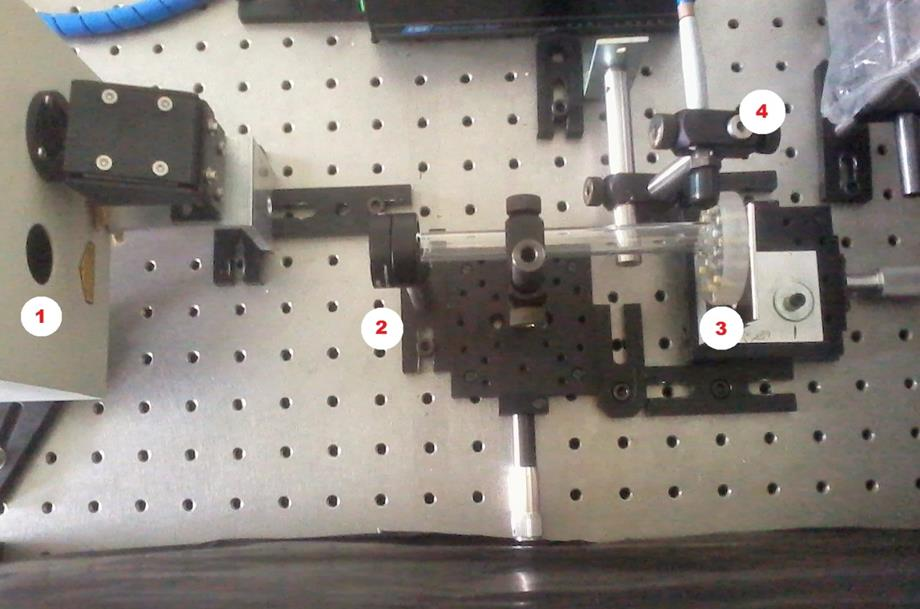
\includegraphics[width=15cm]{Setup LIBS.jpg}
    \caption{\textbf{Equipamiento utilizado en mediciones.} 1) Láser pulsado 2) Lente de 125mm 3) Porta muestra  4) Fibra óptica}
    \label{fig:LIBS2}
\end{figure}

%como se describe en la Figura \ref{fig:dir}
Los archivos están almacenados en una estructura de directorios. Cada grupo (carpetas \textit{04\_02}, \textit{05\_01}, \textit{09\_02}, \textit{12\_02}) corresponde a un tipo de suelo, del cual se tomaron dos muestras (subcarpetas \textit{M14} y \textit{M2}, \textit{M6} y \textit{M9}, \textit{M13} y \textit{M8}, \textit{M4} y \textit{M8}, dos por cada grupo). Para cada muestra se realizaron mediciones repetidas las cuales fueron almacenadas en la carpeta correspondiente. Cada archivo posee dos columnas, uno correspondiente a las longitudes de onda y el otro a las intensidades observadas.

%\begin{table}[ht]
%\centering
%\begin{tabular}{|c|c|}
%\hline
%Grupo                        & Muestras  \\ \hline
%04\_02                       & M14, M2       \\ \hline
%05\_01                       & M6, M9        \\ \hline
%09\_02                       & M13, M8       \\ \hline
%12\_02                       & M4, M5        \\ \hline
%\end{tabular}
%\caption{\textbf{Estructura de directorios}}
%\label{table:folder}
%\end{table}

%\begin{figure}[htbp]
%\centering
%\framebox[\textwidth]{%
%\noindent\hspace{0.3\linewidth}\begin{minipage}{0.5\textwidth}
%    \dirtree{%
%    .1 spc24Oct2019.
%    .2 04\_02.
%    .3 M14.
%    .3 M2.
%    .2 05\_01.
%    .3 M6.
%    .3 M9.
%    .2 09\_02.
%    .3 M13.
%    .3 M8.
%    .2 12\_02.
%    .3 M4.
%    .3 M5.
%    }
%\end{minipage}
%}
%\caption{Directorio de archivos}
%\label{fig:dir}
%\end{figure}

\section{Métodos}
\subsection{Preprocesamiento}
\subsubsection{Ordenado de datos}
El conjunto de datos en su forma original fue convertido a un solo archivo en un formato estándar donde cada fila corresponde a uno de los espectros y cada columna es una variable, con el propósito de facilitar la aplicación de los diversos algoritmos utilizados en este trabajo (incluidos aquellos empleados durante el análisis exploratorio). Se añadieron variables que identifican el archivo original del espectro, a que muestra y tipo de suelo pertenecen, para complementar a las variables correspondientes a la intensidad en cada longitud de onda, como puede verse en el Cuadro \ref{table:tidy}.

\begin{table}[ht]
\centering
\begin{tabular}{|c|c|c|c|c|c|}
\hline
%\multicolumn{6}{l}{Minería.csv} \\ \hline
Grupo    & Muestra     & Archivo & 293,83nm & $\cdots$ & 729,06nm \\ \hline
Grupo archivo 1    & Muestra archivo 1     & Archivo 1 & $I_{1,1}$ & $\cdots$ & $I_{7800,1}$ \\ \hline
Grupo archivo 2    & Muestra archivo 2     & Archivo 2 & $I_{1,2}$ & $\cdots$ & $I_{7800,2}$ \\ \hline
$\vdots$ & $\vdots$ & $\vdots$ & $\vdots$ & $\cdots$ & $\vdots$ \\ \hline
Grupo archivo 156    & Muestra archivo 156 & Archivo 156 & $I_{1,156}$ & $\cdots$ & $I_{7800,156}$ \\ \hline
\end{tabular}
\caption{\textbf{Estructura del archivo procesado}}
\label{table:tidy}
\end{table}

\subsection{Análisis exploratorio de datos}
\subsubsection{Frecuencias}

El conjunto de datos está mayoritariamente balanceado. Hay 20 espectros por muestra y 40 por grupo (con excepción de la muestra M6 para el cual hay disponibles 16 espectros). 

%\begin{figure}[htbp]
%    \centering
    %\captionsetup{justification=centering}
%    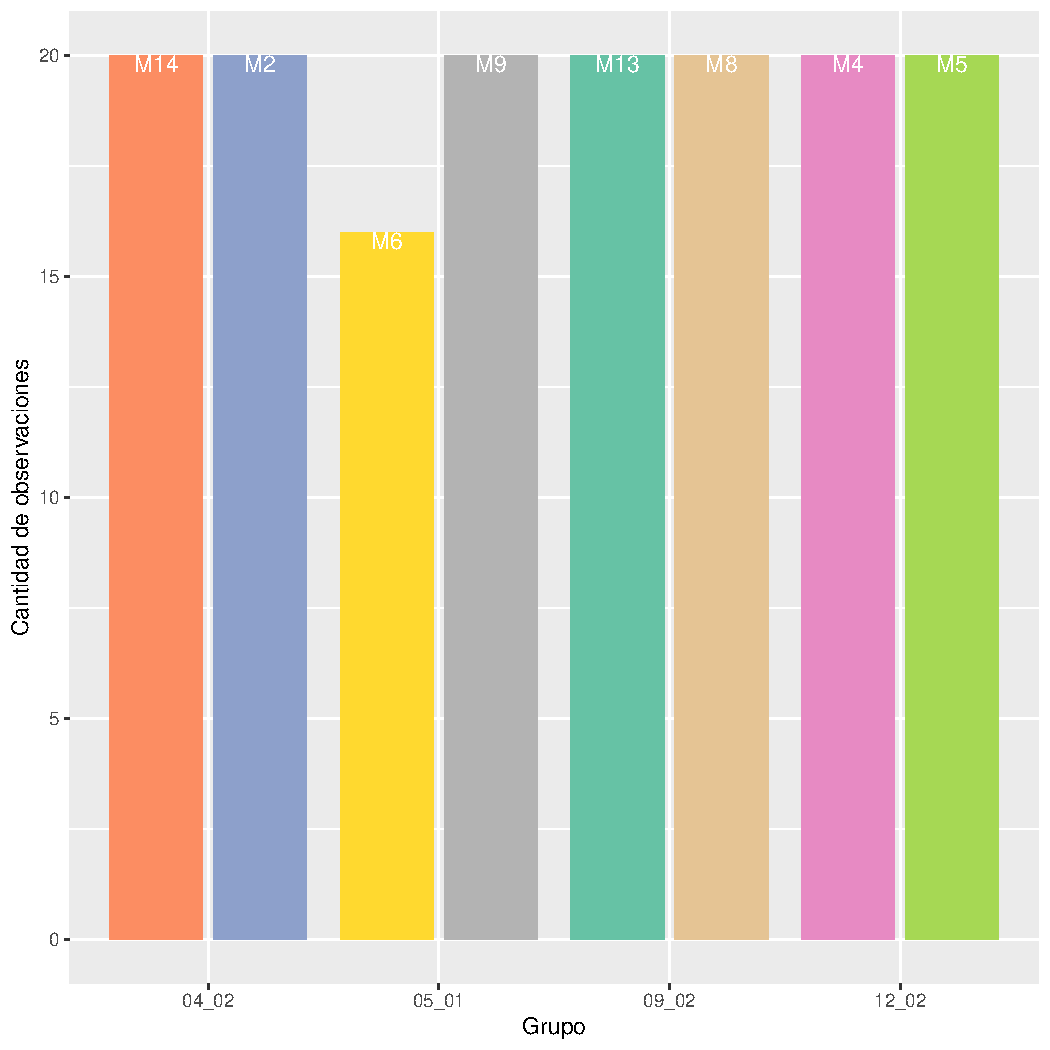
\includegraphics[width=10cm]{Class_distribution.pdf}
%    \caption{\textbf{Frecuencia de observaciones por tipo de suelo y muestra. }}
%    \label{fig:class}
%\end{figure}

\subsubsection{Visualización espectros}

Pueden verse espectros medianos de cada tipo de suelo (obtenidos calculando la mediana de la intensidad de cada longitud de onda y mapeando las variables de longitud de onda al eje horizontal y las intensidades correspondientes a cada una al eje vertical) en la Figura \ref{fig:samples}. 

Puede apreciarse que cada grupo tiene un espectro distintivo que permite diferenciarlos entre sí. Por ejemplo, los grupos \textit{04\_02} y \textit{09\_02} tienen picos de mayor intensidad en todas las longitudes de onda comparados con otros tipos de suelo, \textit{09\_02} tiene mayor intensidad que \textit{04\_02} en (aproximadamente) 480nm y 600nm así como 340nm, mientras que \textit{05\_01} muestra mayor intensidad que \textit{12\_02} en la región entre 500nm y 600nm.

%considerar corregir imágenes
\begin{figure}[htbp]
    \centering
    %\captionsetup{justification=centering}
    \begin{subfigure}[b]{0.45\textwidth}
        \caption{Grupo 04\_02}
        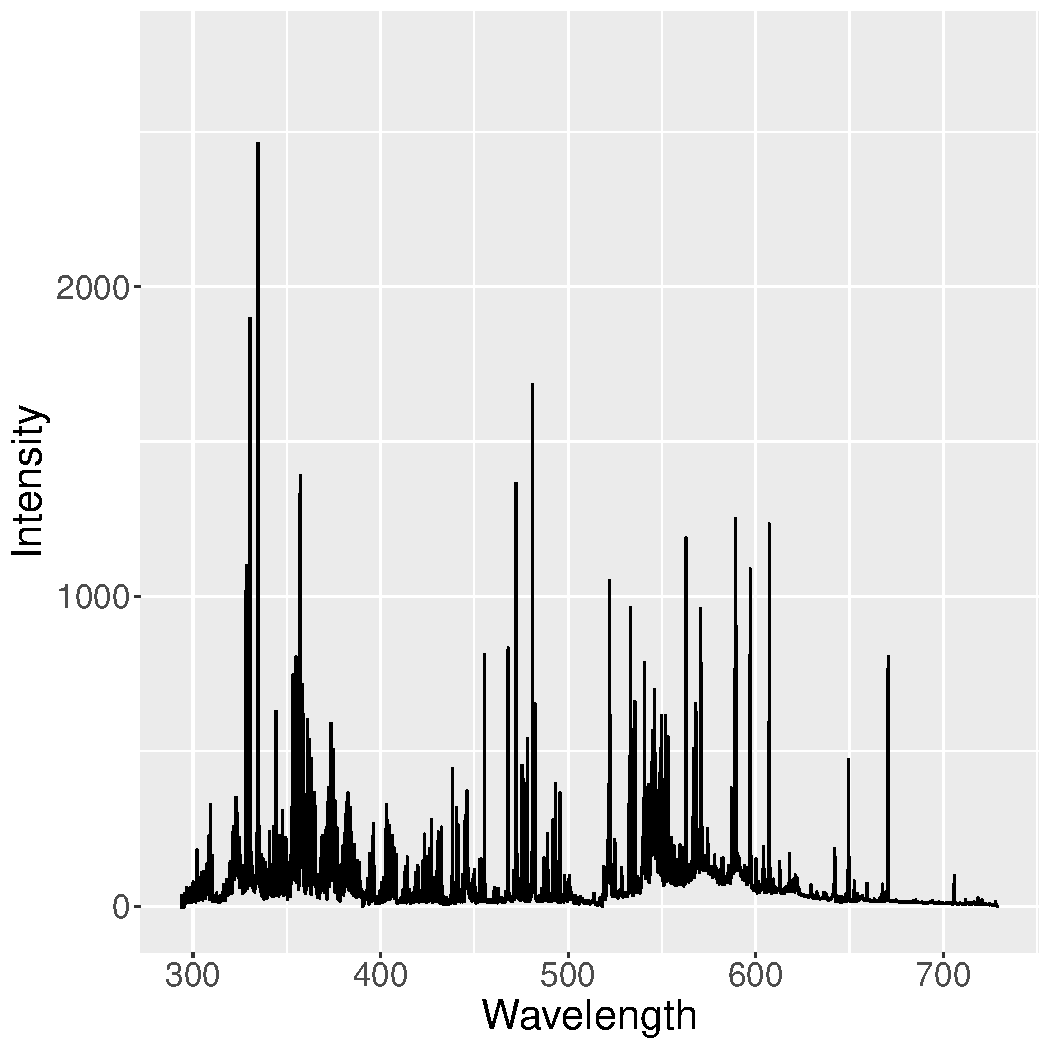
\includegraphics[width=\textwidth]{median_04_02.pdf}
    \end{subfigure}
    \begin{subfigure}[b]{0.45\textwidth}
        \caption{Grupo 05\_01}
        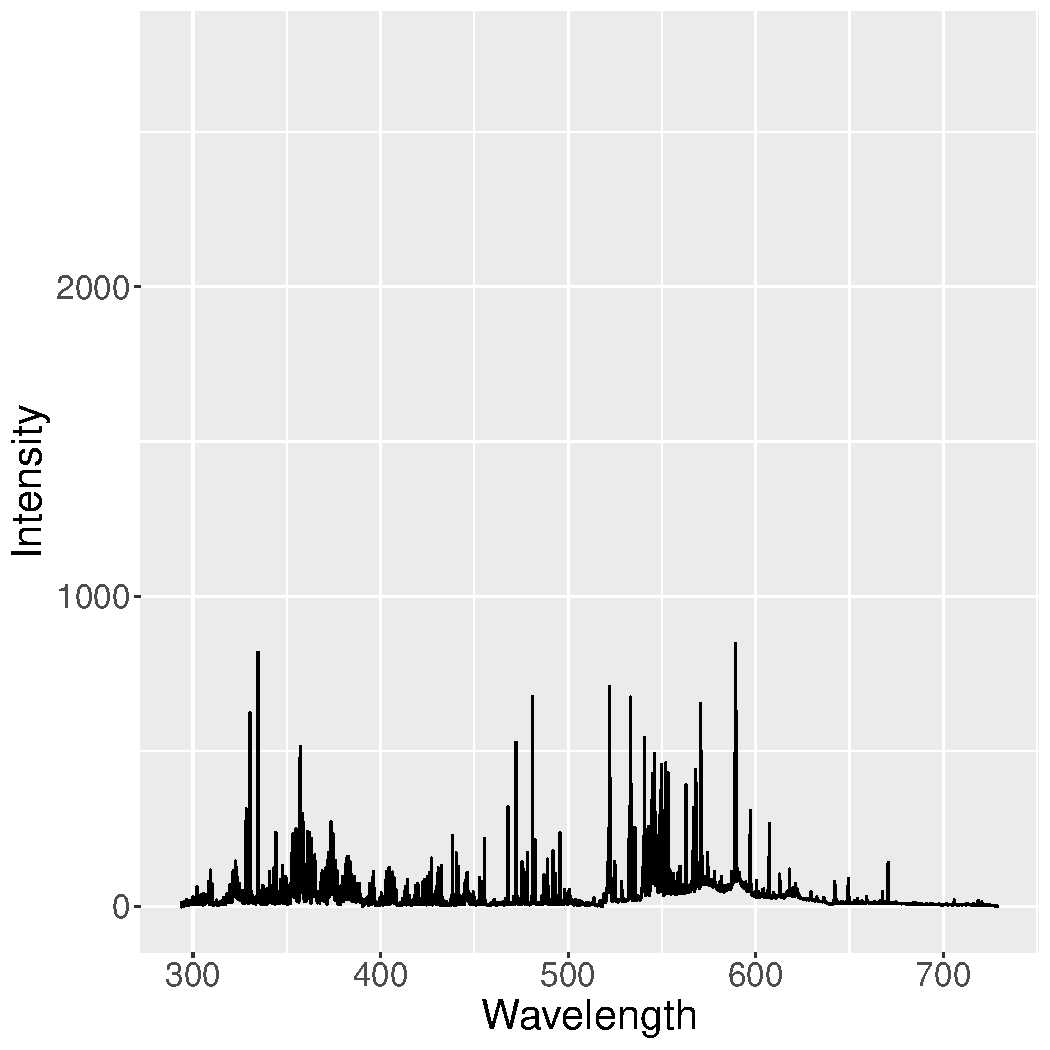
\includegraphics[width=\textwidth]{median_05_01.pdf}
    \end{subfigure}
    \begin{subfigure}[b]{0.45\textwidth}
        \caption{Grupo 09\_02}
        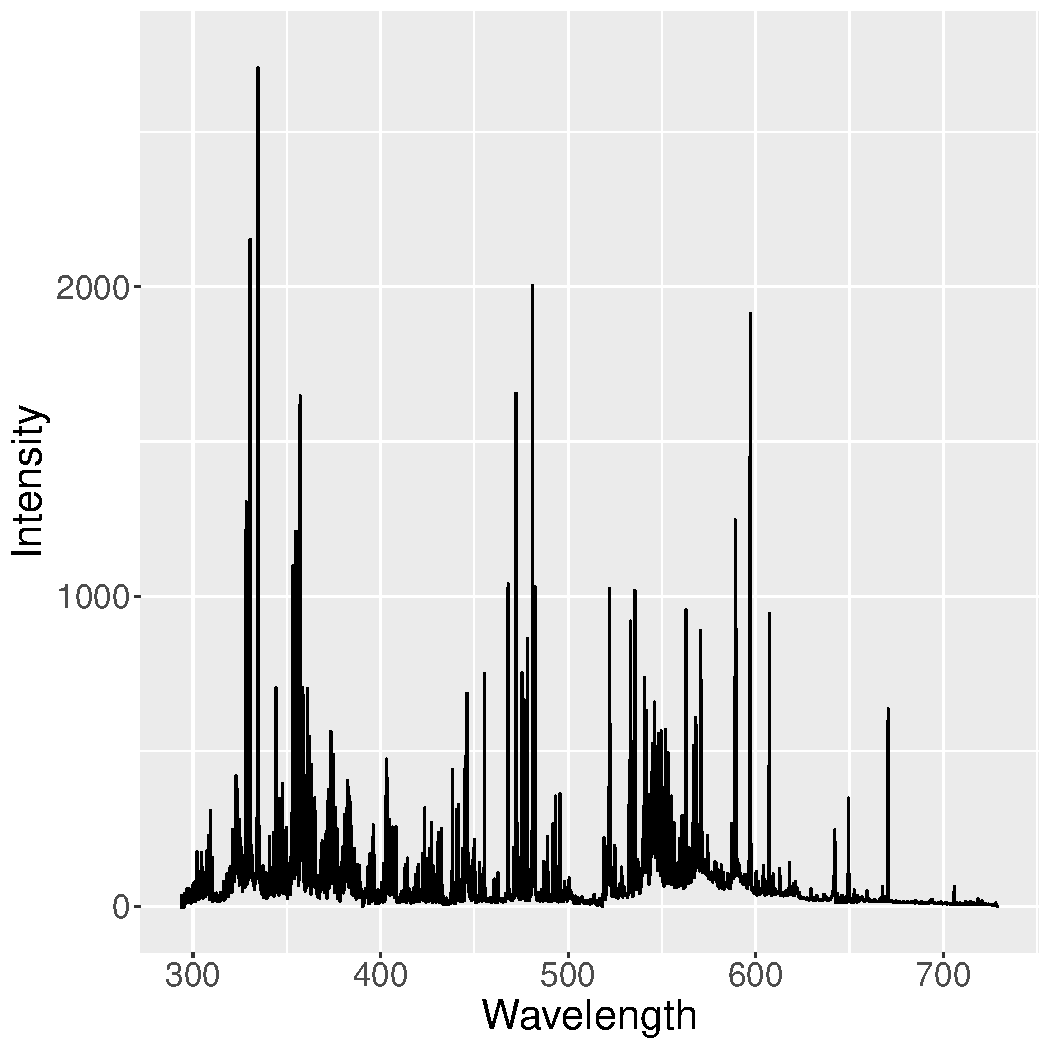
\includegraphics[width=\textwidth]{median_09_02.pdf}
    \end{subfigure}
    \begin{subfigure}[b]{0.45\textwidth}
        \caption{Grupo 12\_02}
        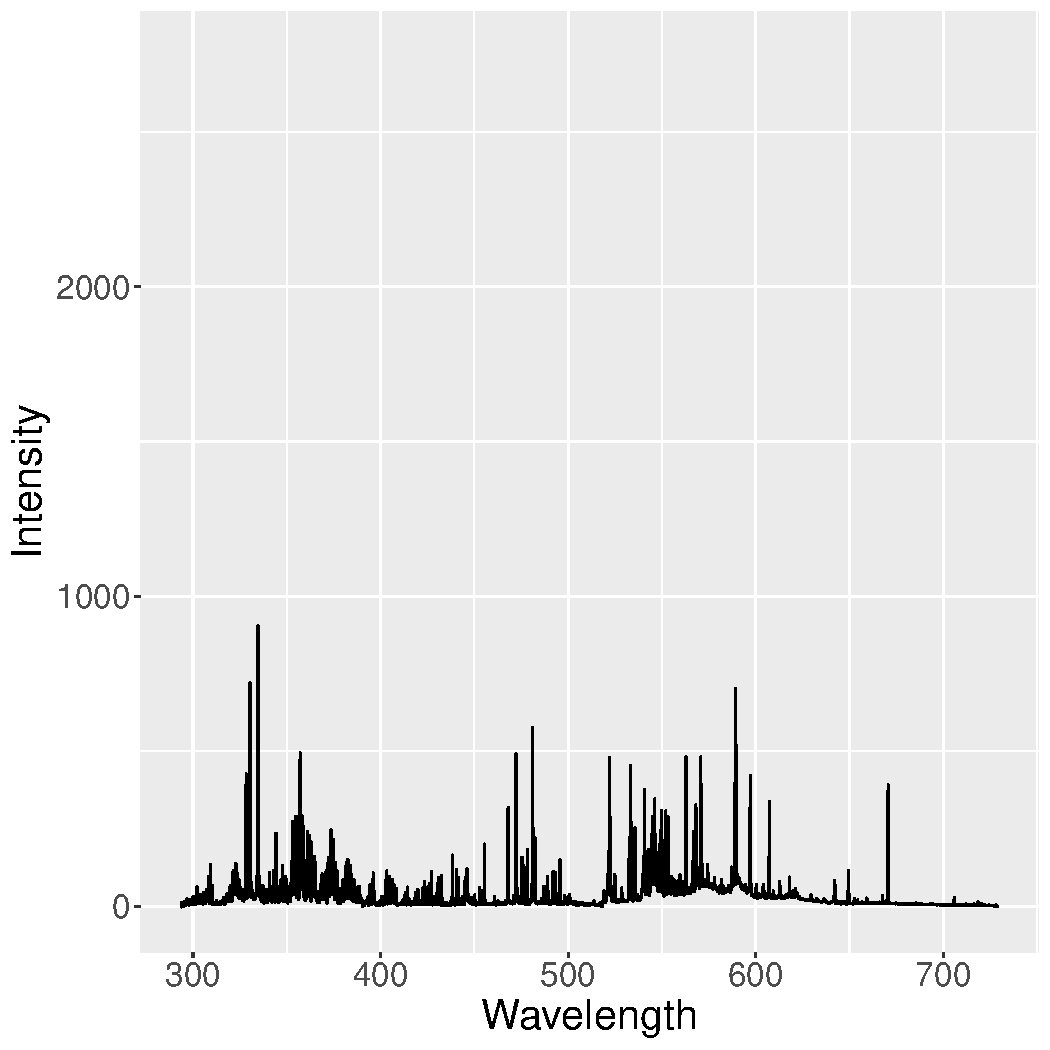
\includegraphics[width=\textwidth]{median_12_02.pdf}
    \end{subfigure}
    \caption{\textbf{Espectro mediano de cada tipo de suelo}.}  
    \label{fig:samples}
\end{figure}

\subsubsection{Tests}

%https://www.ncbi.nlm.nih.gov/pmc/articles/PMC3927875/
%https://arxiv.org/pdf/1904.05289.pdf
%https://www.tandfonline.com/doi/abs/10.1080/03610918.2015.1089286?journalCode=lssp20
%https://www.sciencedirect.com/science/article/pii/S0167947309001704
%Article Normality Testing of High-dimensional Data Based on Principle Component and Jarque–Bera Statistics
Para probar algunos de los supuestos necesarios en este trabajo, se realizó un test de Henze-Zirkler para determinar si cada grupo de muestras sigue una distribución normal multivariada, cuyos resultados pueden verse en el Cuadro \ref{table:normality}. Luego se realizó un test de Levene para ver si se verifica la homocedasticidad, la cuál fue rechazada para $\alpha = 0,05$ ($F = 7,38, p-valor = 0,00012$).

%04_02    (160, nan, False)
%05_01    (144, nan, False)
%09_02    (160, nan, False)
%12_02    (160, nan, False)

%Group
%04_02    (160, nan, False)
%05_01    (144, nan, False)
%09_02    (160, nan, False)
%12_02    (160, nan, False)

%(7.38, 0.00012 ,False)

\begin{table}[htbp]
\centering
\begin{tabular}{|c|c|c|c|}
\hline
Grupo                        & HZ & p-valor & Normal ($\alpha = 0,05$) \\ \hline
04\_02                       & 160 & $\sim$0 & Falso      \\ \hline
05\_01                       & 144 & $\sim$0 & Falso       \\ \hline
09\_02                       & 160 & $\sim$0 & Falso      \\ \hline
12\_02                       & 160 & $\sim$0 & Falso       \\ \hline
\end{tabular}
\caption{\textbf{Resultados de test de normalidad multivariada}.}
\label{table:normality}
\end{table}

La violación de estos supuestos no resulta ser un problema severo en la práctica para los métodos utilizados en este trabajo pero debe tenerse en consideración.

\subsubsection{Análisis de componentes principales}

Las aplicaciones de espectroscopía suelen involucrar variables altamente correlacionadas. Esto permite que el PCA sea bastante efectivo para representar datos de esta variedad en un espacio de menor dimensionalidad. En este tipo de aplicaciones no suele estandarizarse los datos debido a que los niveles de energía de los picos y no solo sus variaciones poseen cierta información sobre la composición química de la muestra, y a que el ruido es representado en una menor escala de esta forma.

Aparte de ello, al ser esta una transformación una rotación de los datos originales, se conservan las relaciones de distancias entre los distintos espectros en el espacio original, por lo que puede verse cúmulos correspondientes a cada grupo en la Figura \ref{fig:pca}.

\begin{figure}[htbp]
    \centering
    %\captionsetup{justification=centering}
    \begin{subfigure}[b]{0.9\textwidth}
        \caption{}
        \includesvg[width=\textwidth]{PCA1a.svg}
        \label{fig:pca}
    \end{subfigure}
    \begin{subfigure}[b]{0.9\textwidth}
        \caption{}
        \includesvg[width=\textwidth]{PCA1b.svg}
        \label{fig:pcab}
    \end{subfigure}
    \caption{\textbf{Análisis de componentes principales}. a)Clásico b)Robusto}    
\end{figure}

Una dificultad que tiene el PCA en su forma más básica es la sensibilidad a outliers ya que afecta la estimación de covarianzas. Los primeros componentes principales son atraídos hacia los outliers y puede que no se capture apropiadamente la variación de observaciones regulares\cite{Hubert2005}.

Así que se decidió utilizar una variante robusta de PCA introducida por Hubert\cite{Hubert2005}. Este algoritmo obtiene suficientes componentes para explicar un 90\% de la varianza a menos que se lo configure explícitamente para que obtenga un número diferente de componentes (esto se hizo en aquellos casos en donde el algoritmo se quedaba con un solo componente). Puede observarse en la Figura \ref{fig:pcab} que, si bien, salvo una rotación y una cuestión de escalas los resultados no son tan diferentes al PCA clásico, queda en evidencia un solapamiento mayor entre los tipos de suelo \textit{05\_01} y \textit{12\_02} cuando se emplea una baja cantidad de dimensiones.

Otro aspecto que se exploró con esta metodología es si hay diferencias entre las dos muestras de un tipo específico de suelo (esto podría indicar una falta de homogeneidad entre las muestras). Como puede verse en la Figura \ref{fig:grouppca}, los cúmulos correspondientes a muestras del mismo tipo de suelo se mezclan entre sí o son adyacentes, por lo cual las diferencias no son importantes.

\begin{figure}[htbp]
    \centering
    %\captionsetup{justification=centering}
    \begin{subfigure}[b]{0.45\textwidth}
        \caption{Grupo 04\_02}
        \includesvg[width=\textwidth]{PCARG1.svg}
    \end{subfigure}
    \begin{subfigure}[b]{0.45\textwidth}
        \caption{Grupo 05\_01}
        \includesvg[width=\textwidth]{PCARG2.svg}
    \end{subfigure}
    \begin{subfigure}[b]{0.45\textwidth}
        \caption{Grupo 09\_02}
        \includesvg[width=\textwidth]{PCARG3.svg}
    \end{subfigure}
    \begin{subfigure}[b]{0.45\textwidth}
        \caption{Grupo 12\_02}
        \includesvg[width=\textwidth]{PCARG4.svg}
    \end{subfigure}
    \caption{\textbf{Análisis de componentes principales por grupo}, una muestra en negro y la otra en púrpura.}  
    \label{fig:grouppca}
\end{figure}

También puede identificarse outliers dentro de cada grupo mediante gráficos de diagnóstico basados en PCA\cite{PCA}. Esto requiere que los datos regulares tengan una distribución normal multivariada. Se asume que distribuciones de este tipo cubren razonablemente las mismas regiones que los cúmulos de datos observados en la Figura \ref{fig:pcab} de manera de poder usar esta técnica. En ese caso, podemos identificar tres tipos de outliers: aquellos que mayoritariamente yacen en el subespacio generado por $K$ componentes principales pero que están lejos de las observaciones regulares, aquellas que tengan una componente ortogonal al subespacio generado por las componentes principales de magnitud importante y aquellas cuyas proyecciones al subespacio están lejos de las observaciones regulares y también poseen una componente ortogonal importante. 

Estos se identifican mediante dos tests: uno basado en un puntaje de distancia robusto $SD$ (distancia de Mahalanobis respecto del centro de cada cúmulo en el subespacio generado por $K$ componentes principales): 
\begin{equation}
SD = \sqrt{\sum_{p = 1}^K \frac{t_p^2}{\lambda_p}}    
\end{equation} 
donde $t_p$ son las coordenadas de una observación $\mathbf{x}$ en el espacio de componentes principales y $\lambda_p$ son los autovalores de la matriz covarianza robusta, con un punto de corte en $\sqrt{\chi_{K,0,975}^2}$,  y otro basado en la distancia ortogonal al subespacio de componentes principales $OD$:
\begin{equation}
OD = ||\mathbf{x} - \hat{\mu} - \mathbf{t} \mathbf{V}^T_K||    
\end{equation}
donde $\hat{\mu}$ es el centro del cúmulo y $\mathbf{V}_K$ contiene los primeros $K$ componentes principales, con un punto de corte $(\hat{\mu}_{OD} + \hat{\sigma}_{OD} z_{0,975})^{\frac{2}{3}}$. Los gráficos de diagnóstico para los cuatro tipos de suelo pueden verse en la Figura \ref{fig:diag}. En el Cuadro \ref{table:outliers} se resume las anomalías encontradas en los outliers señalados por los gráficos de diagnóstico (obtenidos mediante análisis similares al que puede verse en el Anexo A).

\begin{figure}[htbp]
    \centering
    %\captionsetup{justification=centering}
    \begin{subfigure}[b]{0.45\textwidth}
        \caption{Grupo 04\_02}
        \includesvg[width=\textwidth]{diagplotG1.svg}
    \end{subfigure}
    \begin{subfigure}[b]{0.45\textwidth}
        \caption{Grupo 05\_01}
        \includesvg[width=\textwidth]{diagplotG2.svg}
    \end{subfigure}
    \begin{subfigure}[b]{0.45\textwidth}
        \caption{Grupo 09\_02}
        \includesvg[width=\textwidth]{diagplotG3.svg}
    \end{subfigure}
    \begin{subfigure}[b]{0.45\textwidth}
        \caption{Grupo 12\_02}
        \includesvg[width=\textwidth]{diagplotG4.svg}
    \end{subfigure}
    \caption{\textbf{Gráficos de diagnóstico por grupo}. Incluye líneas de corte para las distancias ortogonales y en el subespacio de componentes principales}  
    \label{fig:diag}
\end{figure}

\begin{table}[htbp]
\centering
\begin{tabular}{|c|p{0.1\linewidth}|c|p{0.19\linewidth}|p{0.5\linewidth}|}
\hline
Grupo & N°outlier & Muestra & Archivos & Tipos de outlier \\ \hline
\multirow{2}{3em}{04\_02} & 4, 13, 17 & M14 & M14\_04, M14\_13, M14\_17 & Picos de mayor intensidad, Sin identificar, Picos de menor intensidad \\ \cline{2-5}
& 37 & M2 & M2\_17 & Sin identificar \\ \hline
\multirow{2}{3em}{05\_01} & 2, 4, 5, 9 & M6 & M6\_02, M6\_04, M6\_05, M6\_09 & Picos de alta intensidad, Picos de alta intensidad, Picos de alta intensidad entre 500nm y 550nm, Picos de alta intensidad \\ \cline{2-5}
& 24, 26, 30, 31 & M9 & M9\_08, M9\_10, M9\_14, M9\_15  & Sin identificar, Picos de alta intensidad y ruido, Picos de alta intensidad, Pico de alta intensidad en 600nm \\ \hline
\multirow{2}{3em}{09\_02} & 12 & M13 & M13\_12 & Picos de menor intensidad \\ \cline{2-5}
& 32 & M8 & M8\_12 & Picos de mayor intensidad \\ \hline
\multirow{2}{3em}{12\_02} & 18 & M4 & M4\_18 & Sin identificar \\ \cline{2-5}
& 28, 29, 30, 33, 36 & M5 & M5\_08, M5\_09, M5\_10, M5\_13, M5\_16 & Picos de alta intensidad en 475nm, Picos de alta intensidad y uno nuevo en 325nm, Picos de alta intensidad y algunos nuevos, Picos de alta intensidad, Picos de alta intensidad y algunos nuevos  \\ \hline
\end{tabular}
\caption{\textbf{Identificación de outliers}}
\label{table:outliers}
\end{table}

Una examinación visual de los outliers no muestra errores groseros de medición, lo cual hace sospechar que el pequeño desbalance entre el número de espectros por muestra es debido a que algunas mediciones fueron descartadas.

El PCA robusto sin los outliers puede verse en la Figura \ref{fig:pca2}. En este caso los cúmulos de observaciones están mejor separados, lo que permite confiar más en el diagnóstico realizado (era más probable que los outliers ocuparan el espacio de otros grupos, se obtienen mejores clústeres removiéndolos).

\begin{figure}[htbp]
    \centering
    \includesvg[width=14cm]{PCA2.svg}
    \caption{\textbf{PCA removiendo outliers.}}
    \label{fig:pca2}
\end{figure}

%\subsubsection{Importancia de variables}
%considerar moverlo a la parte de resultados
%Se utilizó el algoritmo \textit{LightGBM} de forma preeliminar (con hiperparámetros en sus valores por defecto) para asignar un puntaje a cada variable correspondiente a las longitudes de onda según cuán relevantes son para entrenar un clasificador que discrimine entre los distintos tipos de suelo. La ubicación de estas variables para espectros representativos de cada grupo puede verse en la Figura. Se observa que las variables encontradas tiene cierta relación con los picos de energía observados.


\subsection{Reducción dimensional}

Antes de entrenar un clasificador, es conveniente aplicar procedimientos de reducción dimensional en los datos, ya sea para reducir los tiempos de entrenamiento y la complejidad de los modelos obtenidos, reducir el efecto del ruido y lidiar con el problema de colinearidad en los espectros químicos. Las técnicas utilizadas en este trabajo son no supervisadas.

Los algoritmos empleados con este propósito fueron:

\begin{itemize}
  \item PCAR: el algoritmo robusto empleado durante la exploración del conjunto de datos también fue utilizado de esta forma. Se buscó extraer la mayor cantidad de componentes principales posibles y almacenarlos en un nuevo archivo para su uso posterior, pero por una cuestión de estabilidad numérica del algoritmo solo se tomaron 90 componentes.
  \item SOM: esta red neuronal genera una representación bidimensional de los datos preservando la estructura topológica. Un gráfico de la proyección de los datos resulta en una grilla cuadrada o rectangular. Los hiperparámetros fueron elegidos siguiendo las propuestas de Tian\cite{Tian2014} y Riese\cite{SuSi} y confirmando visualmente que se obtuvo una proyección sin fallas importantes: una tasa de aprendizaje de $0,3$, una función de vecindad gaussiana, $\sigma = 1$, decaimiento asintótico, una distancia de activación euclidea, una topología rectangular y $10X10$ neuronas (Tian recomienda usar $5 \sqrt{N_{muestras}}$ neuronas). Se recomienda una cantidad considerable de iteraciones de entrenamiento (al menos 10000).El mapa obtenido puede verse en la Figura \ref{fig:SOM}.
  \item UMAP: esta técnica aprende la estructura de variedad presente en los datos mediante un grafo y lo mapea a un grafo en otro espacio de menor cantidad de dimensiones. La proyección con los hiperparámetros por defecto produce clústeres razonables, como puede verse en la Figura \ref{fig:UMAP}
\end{itemize}

\begin{figure}[htbp]
    \centering
    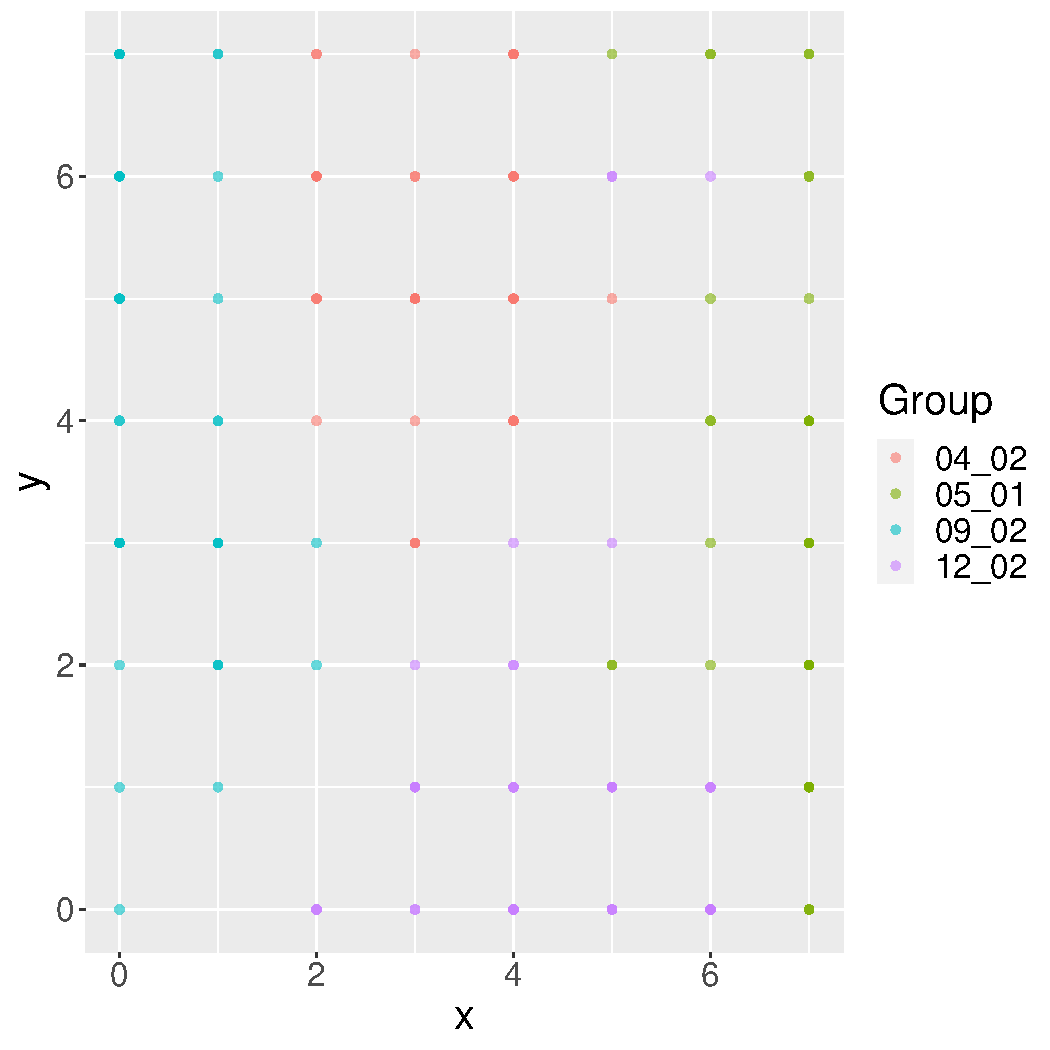
\includegraphics[width=10cm]{SOM.pdf}
    \caption{\textbf{Mapa obtenido mediante SOM.}}
    \label{fig:SOM}
\end{figure}

\begin{figure}[htbp]
    \centering
    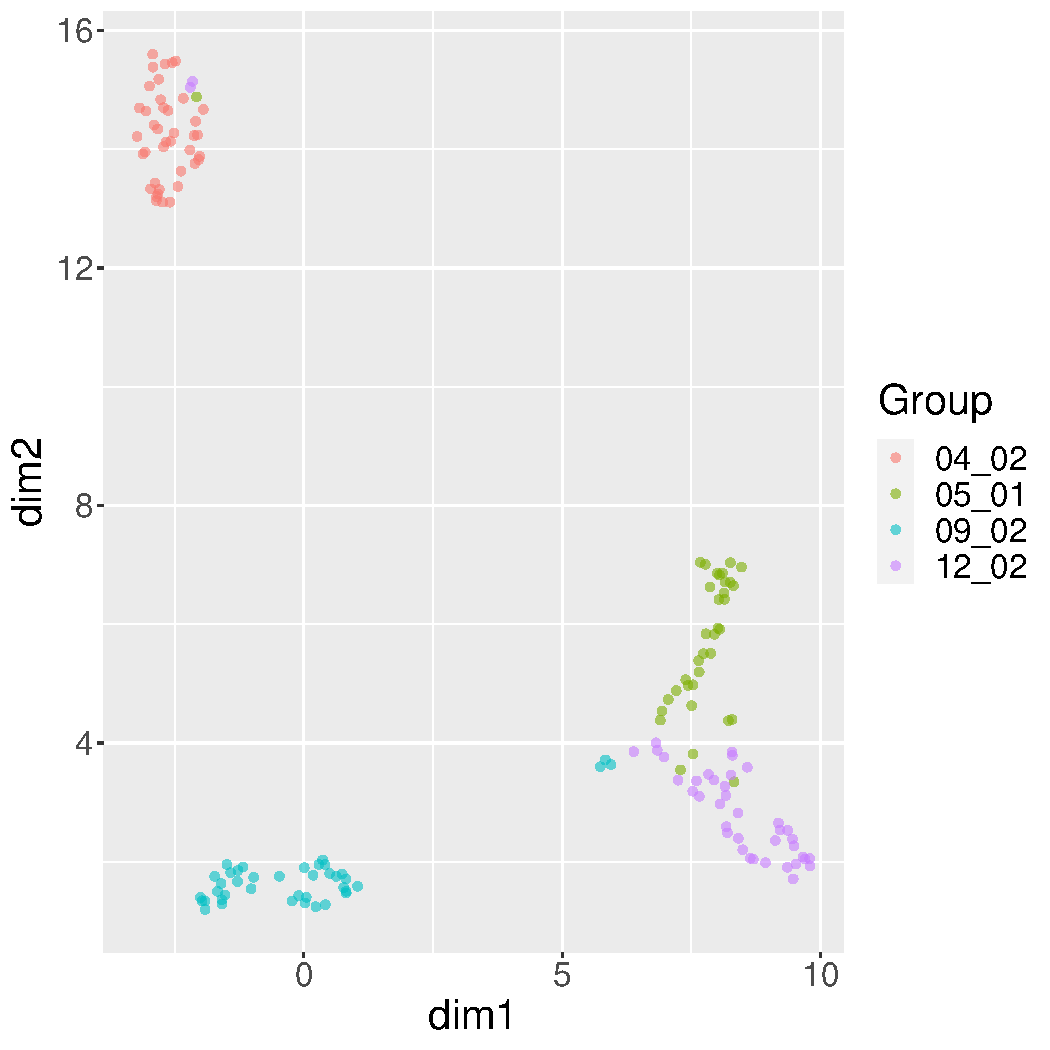
\includegraphics[width=10cm]{UMAP.pdf}
    \caption{\textbf{Mapa obtenido mediante UMAP.}}
    \label{fig:UMAP}
\end{figure}

\textit{Una limitación de este trabajo fue el hecho de que la reducción dimensional fue hecha sobre todos los datos simultáneamente en vez de realizarlo durante el tiempo de entrenamiento, reduciendo ligeramente la capacidad de generalización de los modelos obtenidos.} En caso de tener que lidiar con nuevas muestras, sería deseable repetir este procedimiento desde cero en vez de simplemente transformar los nuevos datos en base a los transformadores ya entrenados. Sin embargo, dado lo poco costoso que es reentrenar modelos para aplicaciones de esta magnitud, no se considera que sea una limitación importante.

\subsection{Clasificación}
\subsubsection{Estrategia de entrenamiento y métricas de evaluación}
Se separó un 20\% del conjunto de datos para ser utilizado como datos de prueba. En aquellos algoritmos donde se aplica, se utilizó una validación cruzada diviendo los datos de entrenamiento en cinco subconjuntos. Se muestreó aleatoriamente dado que los tipos de suelo están casi balanceados.

Para evaluar la calidad de los modelos generados, se utilizaron matrices de confusión para poder visualizar qué clases se confundieron y en qué forma, así como la exactitud ya que no hay ninguna razón para priorizar si se encontraron verdaderos positivos o cuántos verdaderos positivos fueron actualmente recuperados. La exactitud se calculó en base al promedio de corridas con semillas diferentes (aunque empleando las mismas semillas para diferentes métodos de manera que los resultados sean comparables).

También se midió el tiempo de ejecución para poder comparar los costos de ejecución de cada algoritmo.
%colocar comentario sobre tiempos de entrenamiento y clasificación
\subsubsection{Algoritmos de clasificación}
Un método estadístico clásico para clasificación (y relativamente popular en aplicaciones de espectroscopía) es el análisis discriminante bayesiano. Este mismo modeliza las funciones de densidad de probabilidad condicional de cada clase mediante distribuciones normales con tal de obtener varias funciones lineales con la cual decidir la clase de una observación específica. 

Asumiendo la normalidad y homocedasticidad, se realizó un análisis discriminante lineal (LDA). Relajando la suposición de homocedasticidad, se realizó un análisis discriminante cuadrático (QDA). En ambos casos, el hecho de que no se cumplan las suposiciones no es una desviación tan severa que vuelva inefectivo estos métodos. 

%De hecho, puede mostrarse que, para el caso de LDA, pueden derivarse funciones lineales que difieren a lo sumo por un múltiplo escalar a las del LDA mediante una regresión lineal sin realizar ninguna de estas suposiciones\cite{ESL2008} (lo cual da una intuición de por qué funciona en estas situaciones si es posible separar los datos mediante hiperplanos de forma razonable). QUIZÁS MOVERLO A DISCUSIONES

Dado que SOM y UMAP generan mapas que no pueden separarse de forma razonable entre clases mediante fronteras lineales o cuadráticas, aparte de las longitudes originales, solo se utilizó PCAR en combinación con LDA y QDA.

Para propósitos de comparación, también se utilizó un método de aprendizaje automático moderno basado en un ensemble de árboles de decisión (LightGBM). Los hiperparámetros que se optimizaron (al trabajar con las variables originales y con PCAR) fueron el número de hojas por árbol (2, 4, 8, 16, 32, 64 y 128) y la mínima cantidad de observaciones por hoja (2,4,8,16 y 32), estos dos en rangos razonables para 156 muestras, así como la fracción de atributos por árbol (entre 0,2 y 1) y la tasa de aprendizaje (entre 0,005 y 0,3), los cuáles están en la vecindad de los parámetros por defecto del algoritmo. 

Al usar LightGBM en combinación con SOM y UMAP esto no fue suficiente para obtener resultados deseables debido al sobreajuste, así que la fracción de atributos se cambió a 0,5 y 1, y la mínima cantidad de observaciones por hoja se aumentó a 16,20,24,28,32 y 36. Con UMAP específicamente fue necesario ir más lejos y usar un rango inferior en la tasa de aprendizaje (0,005 a 0,1) y hacer una regularización $L_1$ ($\alpha$ es igual a 0, 0,05, 0,1 o 0,15). 

Tanto con métodos estadísticos como de aprendizaje automático, no solo se utilizaron las longitudes de onda sin procesar, sino que también se usaron los algoritmos en combinación con algunos de los conjuntos de datos resultantes tras aplicar los diferentes algoritmos de reducción dimensional.

Un subproducto del uso de LightGBM es una medida de la importancia de atributos para clasificación. En el caso de usar los datos originales, esta medida es en parte informativa de cuáles son las longitudes de onda más relevantes. Una vez entrenado el clasificador con los atributos originales, se visualizó las importancia en función de las longitudes de onda.

\section{Resultados}

Los tiempos de entrenamiento de los algoritmos de reducción dimensional pueden verse en el Cuadro \ref{table:dimensional_reduction}. SOM en particular resulta lo más costoso de ejecutar (y esto no considera el hecho de que puede requerirse varias corridas para ajustar los hiperparámetros adecuadamente).

\begin{table}[htbp]
\centering
\begin{tabular}{|c|c|c|}
\hline
Algoritmo                        & Tiempo promedio[s] & Notas \\ \hline
PCAR                      & 8,676014 & 90 componentes      \\ \hline
UMAP                       & 2.841912 & Hiperparámetros por defecto \\ \hline
SOM                       & 280.322036 & -      \\ \hline
\end{tabular}
\caption{\textbf{Desempeño de algoritmos de reducción dimensional}.}
\label{table:dimensional_reduction}
\end{table}

Los tiempos de entrenamiento y exactitudes promedio de los algoritmos de clasificación para diferentes configuraciones pueden verse en el Cuadro \ref{table:classifier}. 

En el caso de QDA era imposible usar los datos sin aplicar una reducción dimensional (el algoritmo prohibe utilizar variables colineales por una cuestión de estabilidad numérica). 

Los tiempos de entrenamiento para LightGBM con hiperparámetros optimizados consideran el tiempo de una corrida búsqueda de hiperpárametros. En la práctica se necesitan varias corridas por no ser obvio qué rango de hiperparámetros debe explorarse (o si se eligieron los correctos) así que los valores son una subestimación del tiempo total que fue necesario para entrenar los modelos.

\begin{table}[htbp]
\centering
\begin{tabular}{|c|c|c|c|}
\hline
Algoritmo  & Exactitud & Tiempo promedio[s] & Notas \\ \hline
LDA      & 0,99375   & 32,114018     & - \\ \hline
LDA      & 0,96875   & 0,042671     & PCAR \\ \hline
QDA      & 0,91250   & 0,023746     & PCAR \\ \hline
LightGBM & 0,96250   & 4,238983     & Hiperparámetros por defecto \\ \hline
LightGBM & 0,96875   & 1400,645764  & Optimizado \\ \hline
LightGBM & 0,93750   & 0,1091893     & PCAR con hiperparámetros por defecto \\ \hline
LightGBM & 0,94375   & 54,161651  & PCAR Optimizado \\ \hline
LightGBM & 0,93750   & 0,072268     & UMAP con hiperparámetros por defecto \\ \hline
LightGBM & 0,94375   & 133,904209  & UMAP Optimizado \\ \hline
LightGBM & 0,96250   & 0,068559     & SOM con hiperparámetros por defecto \\ \hline
LightGBM & 0,96250   & 122,837646  & SOM Optimizado \\ \hline

\end{tabular}
\caption{\textbf{Desempeño de algoritmos de clasificación}.}
\label{table:classifier}
\end{table}

En la Figura \ref{fig:classifier} pueden verse las matrices de confusión para los clasificadores en las semillas con los peores resultados. En principio no puede observarse ninguna clase con más errores que el resto. QDA, LightGBM-PCAR y LightGBM-UMAP son las que muestran los peores desempeños individuales.

\begin{figure}[htbp]
    \centering
    %\captionsetup{justification=centering}
    \begin{subfigure}[b]{0.35\textwidth}
        \caption{LDA}
        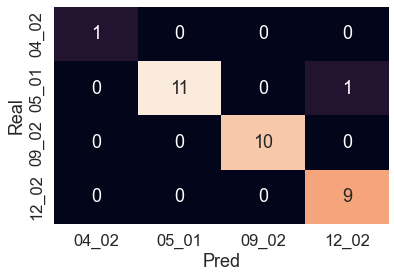
\includegraphics[width=\textwidth]{LDA.png}
    \end{subfigure}
    \begin{subfigure}[b]{0.35\textwidth}
        \caption{LDA-PCAR}
        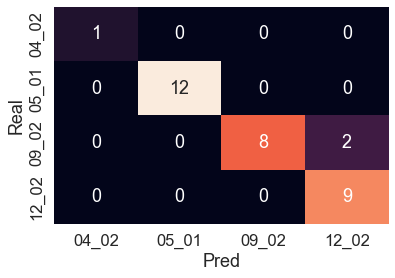
\includegraphics[width=\textwidth]{LDAPCAR.png}
    \end{subfigure}
    \begin{subfigure}[b]{0.35\textwidth}
        \caption{QDA-PCR}
        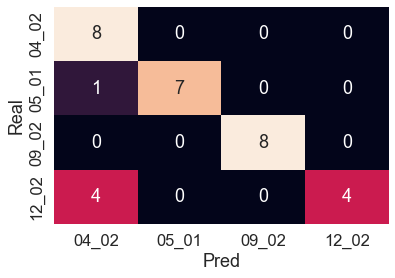
\includegraphics[width=\textwidth]{QDAPCAR.png}
    \end{subfigure}
    \begin{subfigure}[b]{0.35\textwidth}
        \caption{LightGBM por defecto}
        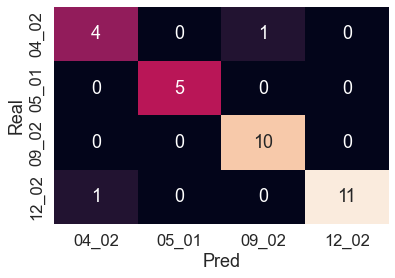
\includegraphics[width=\textwidth]{LightGBMbase.png}
    \end{subfigure}
    \begin{subfigure}[b]{0.35\textwidth}
        \caption{LightGBM optimizado}
        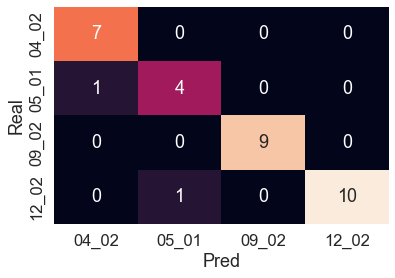
\includegraphics[width=\textwidth]{LightGBMopt.png}
    \end{subfigure}
    \begin{subfigure}[b]{0.35\textwidth}
        \caption{LightGBM-PCAR optimizado}
        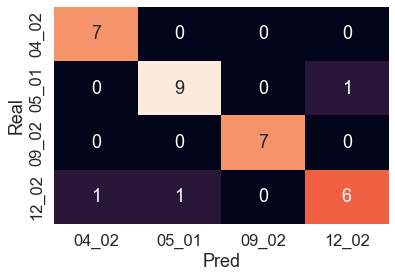
\includegraphics[width=\textwidth]{LightGBMPCARopt.png}
    \end{subfigure}
    \begin{subfigure}[b]{0.35\textwidth}
        \caption{LightGBM-UMAP optimizado}
        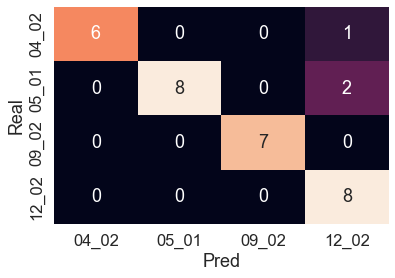
\includegraphics[width=\textwidth]{LightGBMUMAPopt.png}
    \end{subfigure}
    \begin{subfigure}[b]{0.35\textwidth}
        \caption{LightGBM-SOM optimizado}
        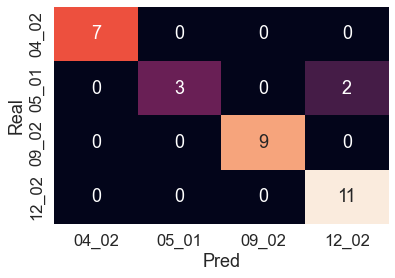
\includegraphics[width=\textwidth]{LightGBMSOMopt.png}
    \end{subfigure}
    \caption{\textbf{Matrices de confusión}. Resultados en prueba con la peor semilla }  
    \label{fig:classifier}
\end{figure}

Por último, en la Figura \ref{fig:feature_importance} puede visualizarse las longitudes más importantes obtenidas por LightGBM tras realizar una optimización de hiperparámetros sobre el conjunto de datos original. Solo algunos de los picos son seleccionados de esta forma, pero así también algunas regiones con menor intensidad de señal e inclusive ruido.

\begin{figure}[htbp]
    \centering
    \includesvg[width=10cm]{feature_importance.svg}
    \caption{\textbf{Importancia de atributos.} Los puntos en rojo sobre el espectro mediano de todas mediciones representan las 150 variables más importantes detectadas por LightGBM}
    \label{fig:feature_importance}
\end{figure}

\section{Discusión}

\subsection{Análisis discriminantes}

LDA es el algoritmo con los mejores resultados de clasificación, inclusive usando las variables originales y a pesar de que se violan todos los supuestos para poder utilizarlo (normalidad, homocedasticidad y no colinearidad). Esto es debido tanto a ciertas características del algoritmo así como de su implementación \cite{DA}.

Recuérdese que el análisis discriminante lineal \textit{bayesiano} se basa en el uso de \textit{funciones discriminantes lineales} derivadas de densidades de probabilidad gaussianas para cada grupo, calculadas sobre una observación (representada por el vector fila $\mathbf{x}$, dado que los datos fueron convertidos a un formato \textit{tidy}), para cada grupo $j$:

\begin{equation} \label{eq:lineal_discriminant}
L_j (\mathbf{x}) = \mathbf{x} \boldsymbol{\Sigma}^{-1} \boldsymbol{\mu}_j^T - \frac{1}{2} \boldsymbol{\mu}_j \boldsymbol{\Sigma}^{-1} \boldsymbol{\mu}_j^T + \log \pi_j
\end{equation}

Donde $\boldsymbol{\Sigma}$ es la matriz covarianza, $\boldsymbol{\mu}_j$ es la media del grupo $j$ y $\pi_j$ es la probabilidad a priori de pertenencia al grupo $j$.  

Se estima el grupo al que pertenece una observación mediante $\hat{G}(\mathbf{x}) = \underset{j}{arg\,max} L_j (\mathbf{x})$. Aquellas regiones donde los discriminantes de diferentes clases son iguales conforman fronteras de decisión lineales.

Es razonable suponer a la luz de los resultados de las diferentes corridas que distribuciones normales pueden aproximar las densidades de cada grupo de observaciones, así como que una estimación de la covarianza agrupada también sea una buena aproximación para las covarianzas de diferentes grupos. Pero sería deseable tener una idea de cuán terrible es asumir esto, y aún no explica adecuadamente qué es lo que ocurre con la colinealidad.

Esta última es un problema signficativo para el algoritmo\cite{NAES2001}, de forma análoga a lo que ocurre en regresión lineal (de hecho, puede pensarse el LDA como regresiones lineales que comparan clases bajo una codificación adecuada\cite{ESL2008}). Si uno observa la autodescomposición del inverso de la matriz covarianza estimada a partir de la matriz de datos $\mathbf{X}$ de dimensiones $NXP$:

\begin{equation} \label{eq:eigendecomposition}
\hat{\boldsymbol{\Sigma}}^{-1} = (\mathbf{V} \boldsymbol{\Lambda} \mathbf{V}^T)^{-1} = \sum_{p = 1}^{P} \mathbf{v}_p (\frac{1}{\lambda_p}) \mathbf{v}_p^T 
\end{equation}

puede observarse que autovalores pequeños (y sus correspondientes autovectores) introducirán inestabilidades numéricas. Esto suele ser el caso con variables muy correlacionadas (estos autovalores corresponderan a dimensiones de ruido), y afectará los coeficientes lineales del discriminante, como puede verse expresando a la Ecuación \ref{eq:lineal_discriminant} en términos de puntajes de componentes principales $\mathbf{t}_p = \mathbf{x} \mathbf{v}_p$ tras centrar los datos:
%Podría ser explicado por: https://math.stackexchange.com/questions/4227454/shrinking-eigenvalues-as-two-columns-become-collinear

\begin{equation} \label{eq:score_space}
\hat{L}_j (\mathbf{t}) = \sum_{p = 1}^{P} \frac{\mathbf{t}_p \bar{\mathbf{t}}_{jp}}{\lambda_p} - \frac{1}{2}\sum_{p = 1}^{P} \frac{\bar{\mathbf{t}}_{jp}^2}{\lambda_p} + \log \pi_j
\end{equation}

donde $\bar{\mathbf{t}}_{jp}$ indica el promedio del puntaje $p$ para el grupo $j$.

Sin embargo, lo que importa del discriminante es su capacidad de diferenciar grupos, no simplemente su estabilidad numérica. La potencia clasificadora se ve afectada más bien dependiendo del tamaño relativo de los puntajes $t_p$ respecto de $\lambda_p$. Resulta ser que las dimensiones de ruido descriptas anteriormente pueden suprimirse con poca pérdida de información (o que al menos que la información perdida es menos problema que la presencia de ruido) y esto aumentará el poder clasificador de los discriminantes al reducirse el efecto del ruido.

Esta reducción dimensional es parte de la implementación del algoritmo utilizado en este trabajo. Esta implementación no solo calcula los discriminantes, sino que previamente realiza un \textit{análisis discriminante canónico} como método de reducción dimensional. Se busca una transformación que maximice la dispersión entre clases mientras que al mismo tiempo minimice la dispersión dentro de cada grupo. Para la matriz de datos $\mathbf{X}$ de $N$ observaciones por $P$ variables, se estima tanto la matriz covarianza $\hat{\boldsymbol{\Sigma}}$ como la matriz covarianza de las medias de las clases $\hat{\boldsymbol{\Sigma}}_B$. La transformación buscada se obtiene mediante los autovectores de $\hat{\boldsymbol{\Sigma}}^{-1}\hat{\boldsymbol{\Sigma}}_B$, y generará un espacio de 
\textit{variables canónicas} (ver Anexo B para una descripción más detallada del algoritmo). 

\textit{La supresión de dimensiones problemáticas correspondientes al ruido se hace en este paso.} Si se toma la autodescomposición de la Ecuación \ref{eq:eigendecomposition} y se suprimen las dimensiones con ruido ($\lambda_p < tol$), se obtendrá la matriz $\hat{\boldsymbol{\Sigma}'}$:

\begin{equation} \label{eq:reduction}
\hat{\boldsymbol{\Sigma}'}^{-1} = (\mathbf{V}' \boldsymbol{\Lambda}' \mathbf{V}'^T)^{-1} = \sum_{p = 1}^{A} \mathbf{v}_p (\frac{1}{\lambda_p}) \mathbf{v}_p^T 
\end{equation}

%Como consecuencia esta restricción, las direcciones deseadas (en el espacio original) se calculan mediante los autovectores de $\hat{\Sigma'}^{-1}\hat{\Sigma}_B$.
%revisar si está bien el orden de factores al final

Las funciones discriminantes resultantes tras transformar los datos al espacio de variable canónicas son afortunadamente sencillas:

\begin{equation} \label{eq:lineal_discriminant_proy}
L_j (\mathbf{x}^{*}) = \mathbf{x}^{*} {\boldsymbol{\mu}^{*}_j}^T - \frac{1}{2} ||\boldsymbol{\mu}^{*}_j||^2 + \log \pi_j
\end{equation}

En consecuencia, es más conveniente estudiar el problema de la normalidad y la homocedasticidad en el espacio transformado. En la Figura \ref{fig:LDAspace} pueden observarse los cuatro cúmulos correspondientes a los datos. Idealmente las distribuciones observadas tendrían intervalos de confianza del 95\% representados por esferas de radio 2 (cada cúmulo debería tener distribución $\mathcal{N}(\boldsymbol{\mu}^{*},I_3)$). Para los grupos 05\_01 y 12\_02 los outliers están algo dispersos, mientras que el grupo 09\_02 muestra una forma elipsoidal. Sin embargo, las clases están muy bien separadas en este espacio, lo cual significa que no se introduciría mucho error aproximando las distribuciones empíricas por distribuciones gaussianas ideales. La fuente del error sería mayoritariamente en aquellas observaciones que están lejos de los centros de los cúmulos y/o cerca de las fronteras de decisión entre clases. La tabla de confusión con el peor resultado observado de LDA en la Figura \ref{fig:classifier} muestra que una observación del grupo 05\_01 fue confundida por una de la clase 12\_02, debido a que estas dos clases son las más cercanas entre sí.

\begin{figure}[htbp]
    \centering
    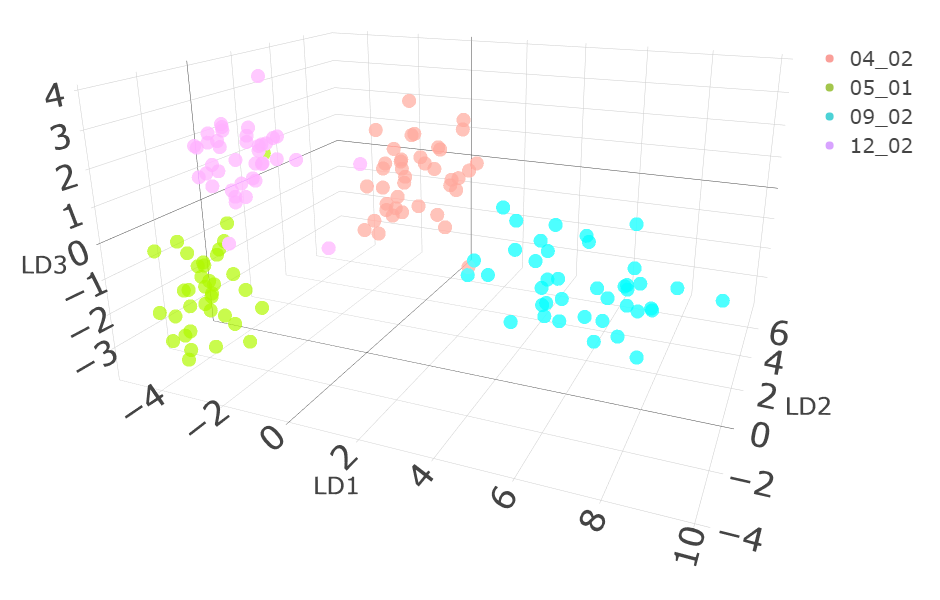
\includegraphics[width=14cm]{LDAspace.png}
    \caption{\textbf{Espacio de variables canónicas.}}
    \label{fig:LDAspace}
\end{figure}

El caso de las funciones discriminantes cuadráticas no es tan conveniente por comparación. Recuérdese el discriminante cuadrático:

\begin{equation} \label{eq:quadratic_discriminant}
Q_j (\mathbf{x}) = - \frac{1}{2} (\mathbf{x} - \boldsymbol{\mu}_j) \boldsymbol{\Sigma}_j^{-1} (\mathbf{x} - \boldsymbol{\mu}_j)^T  - \frac{1}{2} \log |\boldsymbol{\Sigma}_j| + \log \pi_j
\end{equation}

El fenómeno de autovalores pequeños es un problema también, pero la implementación utilizada ya no aplica los pasos de reducción dimensional como en el caso lineal. Solo se hace la autodescomposición de las matrices covarianza por cada discriminante para evitar calcular inversos. Con $\boldsymbol{\Sigma}_j = \mathbf{V}_j \boldsymbol{\Lambda}_j \mathbf{V}_j^T$, la Ecuación \ref{eq:quadratic_discriminant} es tranformada (calculando $\mathbf{X} \mathbf{V}_j \boldsymbol{\Lambda}_j^{-\frac{1}{2}}$) a:

\begin{equation} \label{eq:quadratic_discriminant_proy}
Q_j (\mathbf{x}^{*}) = - \frac{1}{2} ||(\mathbf{x}^{*} - {\mathbf{\mu}^{*}}_j) ||^2   - \frac{1}{2} \sum_p \log \lambda_{pj} + \log \pi_j
\end{equation}

Necesariamente hay que realizar un PCA antes de poder realizar un QDA, y se requiere que haya tantas muestras por grupo como variables\footnote{Esto es consecuencia de que, para una matriz de datos de  $j$ centrada $\mathbf{X}_C \in \mathbb{R}^{NXP}$, $rango(\hat{\boldsymbol{\Sigma}}_j) = rango(\mathbf{X}^T_C \mathbf{X}_C) = rango(\mathbf{X}_C) \le \min (N - 1,P)$ y la matriz inversa no existe si la matriz es deficiente en rango.} así que habrá un límite al número de componentes que pueda tomarse. 

No solo no puede hacerse una reducción dimensional, sino que el número de parámetros del discriminante será más alto (aparte de que se tendrá menos observaciones para estimar cada matriz covarianza, lo cual empeorará la calidad de su estimación). Es por esta razón que QDA obtuvo peores predicciones que LDA a pesar de, en principio, ser más flexible como método.

\subsection{LightGBM}

El mejor desempeño de LightGBM fue observado al realizar una optimización de hiperparámetros sobre las variables originales, aunque con un tiempo de ejecución prolongado. Los métodos de reducción dimensional no permitieron una mejor clasificación.

La importancia de variables (como puede visualizarse en la Figura \ref{fig:feature_importance}) permite una interpretación relativamente sencilla del modelo obtenido: algunos de los picos (y algunas regiones con ruido o picos pequeños) son mejores para decidir entre grupos. El hecho de que utilizó algunas regiones con ruido puede que haya puesto un límite a la capacidad de predicción del clasificador.

%\subsection{Mapas auto organizados}

Para SOM, se observa en la Figura \ref{fig:SOM} que se perdió la separación entre los grupos y que observaciones del mismo grupo no necesariamente son adyacentes (hay un clúster bastante notorio de 12\_02 separado del resto). También se observa que el mapa de atributos generado puede subdividirse en rectángulos sin mucha dificultad, así que el uso de ensembles de árboles es bastante natural. Recuérdese que los árboles son funciones de la forma 

\begin{equation}
f(\mathbf{x}) = \sum_{m = 1}^M c_m \mathds{1}_{\mathcal{R}_m}(\mathbf{x})    
\end{equation} 

donde $\mathcal{R}_m$ corresponde a una región rectangular y $\mathds{1}$ es la función indicadora.

Varios intentos por optimizar los hiperparámetros del algoritmo no lograron mejorar los resultados obtenidos por defecto (el cual es competitivo con el uso de variables originales). La composición de los conjuntos de entrenamiento y prueba puede volverse fácilmente un problema. Es casi seguro haciendo suficientes particiones que se genere un conjunto de entrenamiento que no incluya una región específica, especialmente con un número limitado de observaciones. No ayuda que SOM no posee ninguna granularidad ya que sus resultados están ubicados en una grilla. Puede visualizarse el comportamiento del modelo generado por LightGBM y el conjunto de prueba para una de esas particiones en la Figura \ref{fig:BoundarySOM}.

\begin{figure}[htbp]
    \centering
    %\captionsetup{justification=centering}
    \includesvg[width=15cm]{Decision boundary SOM.svg}
    \caption{\textbf{Frontera de decisión para mapas autoorganizados.}}
    \label{fig:BoundarySOM}
\end{figure}

%\subsection{Aproximación y proyección uniforme de variedad}

En el caso de UMAP, Puede verse en la Figura \ref{fig:UMAP} que la proyección realizada crea pequeños clústeres de puntos cercanos a cúmulos principales de otro color, casi seguro correspondientes a los outliers de cada grupo. Es muy fácil sobreajustar un clasificador aprendiendo esos puntos e introduciendo una frontera de decisión complicada. Aparte, dependiendo de cuáles de esos cúmulos entren en el conjunto de entrenamiento se tendrá mayor o menor dificultad generalizando.

Esa es la razón por la cual fue necesario bajar la complejidad del modelo al realizar la búsqueda de hiperparámetros, aumentando la cantidad mínima de observaciones por hoja y añadiendo una regularización $L_1$. También se bajó la tasa de aprendizaje para reducir problemas de divergencia cuando la búsqueda se acerca cada vez más a uno de los mínimos. Puede verse la frontera de decisión del modelo optimizado para una partición específica en la Figura \ref{fig:BoundaryUMAP}.

\begin{figure}[htbp]
    \centering
    %\captionsetup{justification=centering}
    \includesvg[width=15cm]{Decision boundary UMAP.svg}
    \caption{\textbf{Frontera de decisión para aproximación y proyección uniforme de variedad.}}
    \label{fig:BoundaryUMAP}
\end{figure}

En general, podría haber sido mejor si se hubiese hecho una búsqueda de hiperparámetros de los algoritmos de reducción dimensional (por ejemplo, haber utilizado un mayor número de dimensiones para realizar las proyecciones), aunque esto hubiese requerido de integrar el algoritmo a la etapa de validación cruzada, con el consecuente aumento del tiempo de entrenamiento y un tiempo adicional de desarrollo para implementarlo. También podría haber ayudado marginalmente omitir los outliers durante la etapa de entrenamiento, aunque si hubiesen estado presentes en el conjunto de prueba, estos pondrían un límite a la exactitud del clasificador de alguna forma u otra. 

A pesar de todos los problemas descritos en esta sección, SOM y UMAP puede que tengan aplicaciones en clustering, con el propósito de identificar subgrupos dentro de una clase de muestras para poder analizarlos.

\subsection{Efecto del análisis de componentes principales}

Uno de los efectos más confusos observados en este trabajo fue el peor desempeño de todos los algoritmos al combinarlos con PCA robusto. Una explicación sencilla sería que se perdió información al reducir el número de dimensiones, pero en la sección de análisis discriminante se explicó que la implementación utilizada también incluye una reducción dimensional. Algunas otras razones (inclusive contradictorias entre sí) de las cuales se sospechan:

\begin{itemize}
    \item El PCA robusto fue demasiado conservativo, uno de los parámetros ($\alpha$) del algoritmo controla la cantidad de outliers que debería resistir y quizás el valor por defecto descartó demasiadas observaciones.
    \item El uso de muchos componentes fue contraproductivo si no fueron estimados correctamente por cuestiones numéricas y de limitaciones del algoritmo. Se utilizaron muchos porque con el criterio de 90\% de la varianza explicada solo se elegía uno o dos componentes, y porque durante la realización de los experimentos todavía no se comprendía bien el problema de los autovalores pequeños. 
    \item La implementación de LDA suprime los autovalores de $\hat{\boldsymbol{\Sigma}}$ que son más probables que generen problemas númericos durante la etapa en la que se calcula los autovalores de $\hat{\boldsymbol{\Sigma}}^{-1}\hat{\boldsymbol{\Sigma}}_B$ y quizás su criterio de selección de componentes en base a una tolerancia es mucho más razonable que el utilizado en el resto del trabajo. También puede que sea mejor aproximar esa matriz que eliminar dimensiones tras aplicar el PCA.
    \item Es más fácil separar puntos en un espacio de mayor dimensión porque estos necesariamente van a estar más dispersos, en ese sentido quizás fue contraproductivo aplicar una reducción dimensional. Por otra parte, es más probable generar un modelo que sobreajuste de esta forma.
\end{itemize}

\subsection{Comparación general de desempeños}
Los métodos clásicos de clasificación tuvieron mejores resultados (si solo se evalua la clasificación sin considerar los costos de entrenamiento y ejecución) que métodos modernos. Esto es casi seguramente a que los datos espectrales obtenidos no son difíciles de separar en el espacio, especialmente si se tienen las variables originales (porque los datos estarán más dispersos), por lo cual un modelo lineal es suficiente. Los modelos modernos (y también QDA) intercambian sesgo por varianza, o sea, transforman los datos a espacios más complejos y/o buscan fronteras decisión más complejas, pero esto solo induce un mayor error si un modelo simple ya minimizaba el error total casi por completo. 

Otro punto a favor de técnicas tradicionales es que son más fácilmente explicables. No es posible hacer un análisis estadístico detallado como el que se hizo en el caso de análisis discriminante al utilizar LightGBM, UMAP y SOM. Sin embargo, LightGBM al menos permite hacer una estimación (si bien no rigurosa) de cuáles variables permiten diferenciar clases mejor (y al usarse en combinación con UMAP y SOM se puede visualizar los modelos generados). LDA poseen análisis análogo observando los pesos de las variables en cada autovector obtenido pero no son siempre fáciles de interpretar, por eso se lo omitió de este trabajo.

Si se buscase optimizar los tiempos de ejecución, una combinación de PCA y LDA sería la mejor opción, esta opción vence como clasificador a todos los modelos implementados mediante LightGBM a un bajo costo. Los métodos modernos tienen un tiempo de entrenamiento no competitivo si ese fuera el objetivo aplicación.

Es importante tener en mente que estos resultados no son necesariamente aplicables a otros problemas. Algoritmos más complejos podrían ser mucho más razonables si las clases tuvieran una estructura más heterogénea, o si estuvieramos intentando entrenar modelos que generalicen mejor a muestras con importantes diferencias respecto de las utilizadas en el entrenamiento. Por una cuestión de tiempo y recursos, también tendría sentido usar algoritmos de reducción dimensional a pesar de tener el riesgo de perder cierta capacidad de predicción (aunque podrían ser útiles para separar el ruido de la señal presente en los espectros analizados).
\section{Conclusiones}
En este trabajo se entrenaron y compararon clasificadores basados en métodos del aprendizaje estadístico así como metodologías basadas en el aprendizaje automático moderno para clasificar muestras de cuatro tipos de suelo. El método más exitoso fue LDA debido a que la estructura de los datos espectrales permite una separación entre grupos mediante planos.

El uso de LightGBM fue inferior debido a que sus fronteras de decisión más complejas intercambian el sesgo (el cual era mínimo) por más varianza. Reducir la dimensionalidad de los datos en combinación con esta técnica fue contraproductivo debido a que agregaba sus propios problemas: la selección del número de componentes principales no es trivial, UMAP complicó la estructura de los datos al crear pequeños cúmulos muy cerca de cúmulos mayores de otro color, y SOM acortó la distancia entre los datos (aparte de que la falta de granularidad lo vuelve vulnerable si los datos de entrenamiento no cubren ciertas regiones del espacio).

Se analizaron las restricciones que tiene QDA en el número de variables que puede utilizar, la necesidad de estimar mayor cantidad de parámetros y su incapacidad para lidiar con problemas numéricos (al menos para la implementación utilizada). Por otro lado, el análisis del algoritmo de LDA permitió encontrar algunas fortalezas para lidiar con estos mismos problemas.

Adicionalmente se utilizó el PCA robusto para diagnosticar outliers y entender mejor la estructura de los datos utilizados. Su utilización como método de reducción dimensional presenta algunos inconvenientes no del todo entendidos.

Como trabajo futuro, sería deseable estudiar más en detalle el uso de PCA como método de reducción dimensional para entender mejor sus limitaciones, así como también extender el trabajo a conjuntos de datos con estructuras más complicadas en donde los métodos modernos de aprendizaje automático sean más ventajosos. Los ensembles de árboles son hoy en día el estándar para trabajar con datos tabulares pero no tanto para datos espectrales, en vez de usar eso sería recomendable trabajar con redes neuronales.
\section{Código fuente}
Los scripts utilizados en este trabajo pueden verse en el siguiente repositorio:

\url{https://github.com/federicochecozzi/TT1}

\addcontentsline{toc}{section}{Referencias}
\begin{thebibliography}{0}
%revisar citaciones si hay tiempo
%CHEQUEAR POR CONSISTENCIA DE FORMATOS (Spectroscopy)
    \bibitem{Spectroscopy}Freek van der Meer, Near-infrared laboratory spectroscopy of mineral chemistry: A review, International Journal of Applied Earth Observation and Geoinformation, Volume 65, 2018, Pages 71-78/
    \bibitem{LIBS}Wong, D., Bol’shakov, A. A., \& Russo, R. E. (2010). Laser Induced Breakdown Spectroscopy. In Elsevier eBooks (pp. 1281–1287). 
    \bibitem{Chemo}Varmuza, K., \& Filzmoser, P. (2009). Introduction. In: Introduction to Multivariate Statistical Analysis in Chemometrics (p. 15-44). CRC Press.
    \bibitem{STATS}Somorjai, R. L. (2017). Multivariate Statistical Methods. In Elsevier eBooks (pp. 962–966). 
    \bibitem{F-ENG}Ozturk, S., Bowler, A. L., Rady, A., \& Watson, N. (2022). Near-infrared spectroscopy and machine learning for classification of food powders during a continuous process. Journal of Food Engineering, 341, 111339. 
    \bibitem{ML}Ramirez, C. D., Greenop, M., Ashton, L., \& Rehman, I. U. (2021). Applications of machine learning in spectroscopy. Applied Spectroscopy Reviews, 56(8–10), 733–763.
    \bibitem{GA} Lavine, B. K., Davidson, C. J., \& Moores, A. J. (2002). Genetic algorithms for spectral pattern recognition. Vibrational Spectroscopy, 28(1), 83–95. 
    \bibitem{PCA-SVM}Dahlstrand, U., Sheikh, R., Dybelius Ansson, C., Memarzadeh, K., Reistad, N., \& Malmsjö, M. (2019). Extended-wavelength diffuse reflectance spectroscopy with a machine-learning method for in vivo tissue classification. PloS one, 14(10), e0223682. 
    \bibitem{MULT}Mwanga, E. P., Mapua, S. A., Siria, D. J., Ngowo, H. S., Nangacha, F., Mgando, J. P., Baldini, F., Jiménez, M. A., Ferguson, H. J., Wynne, K., Selvaraj, P., Babayan, S. A., \& Okumu, F. O. (2019). Using mid-infrared spectroscopy and supervised machine-learning to identify vertebrate blood meals in the malaria vector, Anopheles arabiensis. Malaria Journal, 18(1). 
    \bibitem{CLUST} Crase, S., \& Thennadil, S. N. (2022). An analysis framework for clustering algorithm selection with applications to spectroscopy. PLOS ONE, 17(3), e0266369. 
    \bibitem{SOM} Shan, P., Li, Z., Wang, Q., He, Z., Wang, S., Zhao, Y., Wu, Z., \& Peng, S. (2021). Self-organizing maps-based generalized feature set selection for model adaption without reference data for batch process. Analytica Chimica Acta, 1188, 339205. 
    \bibitem{EMSLIBS2019} Vrábel, J., Képeš, E., Duponchel, L., Motto-Ros, V., Fabre, C., Connemann, S., Schreckenberg, F., Prasse, P., Riebe, D., Junjuri, R., Gundawar, M. K., Tan, X., Pořízka, P., \& Kaiser, J. (2020). Classification of challenging Laser-Induced Breakdown Spectroscopy soil sample data - EMSLIBS contest. Spectrochimica Acta Part B: Atomic Spectroscopy, 169, 105872. 
    \bibitem{Hubert2005} Hubert, M., \& Rousseeuw, P. J. (2005). ROBPCA: A New Approach to Robust Principal Component Analysis. Technometrics, 47(1), 64–79. 
    \bibitem{PCA}Varmuza, K., \& Filzmoser, P. (2009). Principal Component Analysis. In: Introduction to Multivariate Statistical Analysis in Chemometrics (p. 73-116). CRC Press.
    \bibitem{Tian2014}Tian, J., Azarian, M. H., \& Pecht, M. (2014). Anomaly Detection Using Self-Organizing Maps-Based K-Nearest Neighbor Algorithm. PHM Society European Conference, 2(1).
    \bibitem{SuSi}Riese, F. M. (n.d.). Hyperparameters. Hyperparameters - SuSi 1.2.2 documentation.
    \bibitem{DA}Venables, W.N. \& Ripley, B.D. (2002). Classification. In: Modern Applied Statistics with S. Statistics and Computing (p. 331-351). Springer, New York, NY.
    \bibitem{NAES2001}Næs, T. \& Mevik, B.-H. (2001), Understanding the collinearity problem in regression and discriminant analysis. J. Chemometrics, 15: 413-426.
    \bibitem{ESL2008}Hastie, T., Tibshirani, R. \& Friedman, J. (2009). Linear Methods for Classification. In: The Elements of Statistical Learning (p. 101-138). Springer Series in Statistics. Springer, New York, NY. 
    
\end{thebibliography}

\newpage

\section*{Anexo A: Análisis de outliers}
\addcontentsline{toc}{section}{Anexo A: Análisis de outliers}

A modo de ejemplo de cómo se hace un análisis visual de los outliers encontrados, en la Figura \ref{fig:outlier_analysis} se muestran los espectros del Grupo 04\_04 y el espectro M14\_04. Estos fueron centrados respecto de la media robusta del grupo. Se observa alrededor de los 600nm que hay picos con significativamente mayor intensidad comparados a todos los espectros del grupo. Cerca de los 675nm puede verse un pico que también tiene mayor intensidad, aunque no es una desviación tan dramática respecto del resto.

\begin{figure}[htbp]
    \centering
    %\captionsetup{justification=centering}
    \begin{subfigure}[b]{0.5\textwidth}
        \caption{Espectros del Grupo 04\_02}
        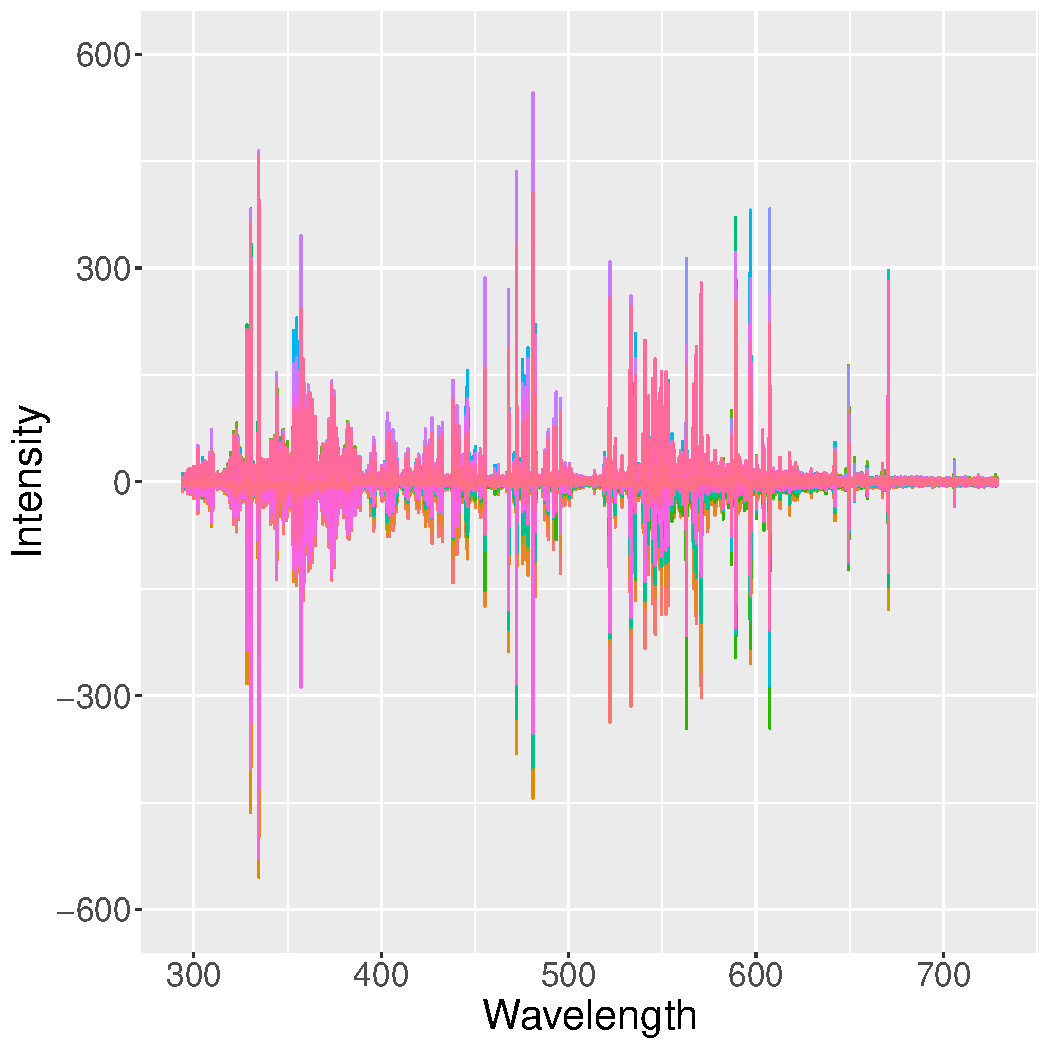
\includegraphics[width=\textwidth]{spectres_centered_04_02b.pdf}
    \end{subfigure}
    \begin{subfigure}[b]{0.5\textwidth}
        \caption{Espectro M14\_04}
        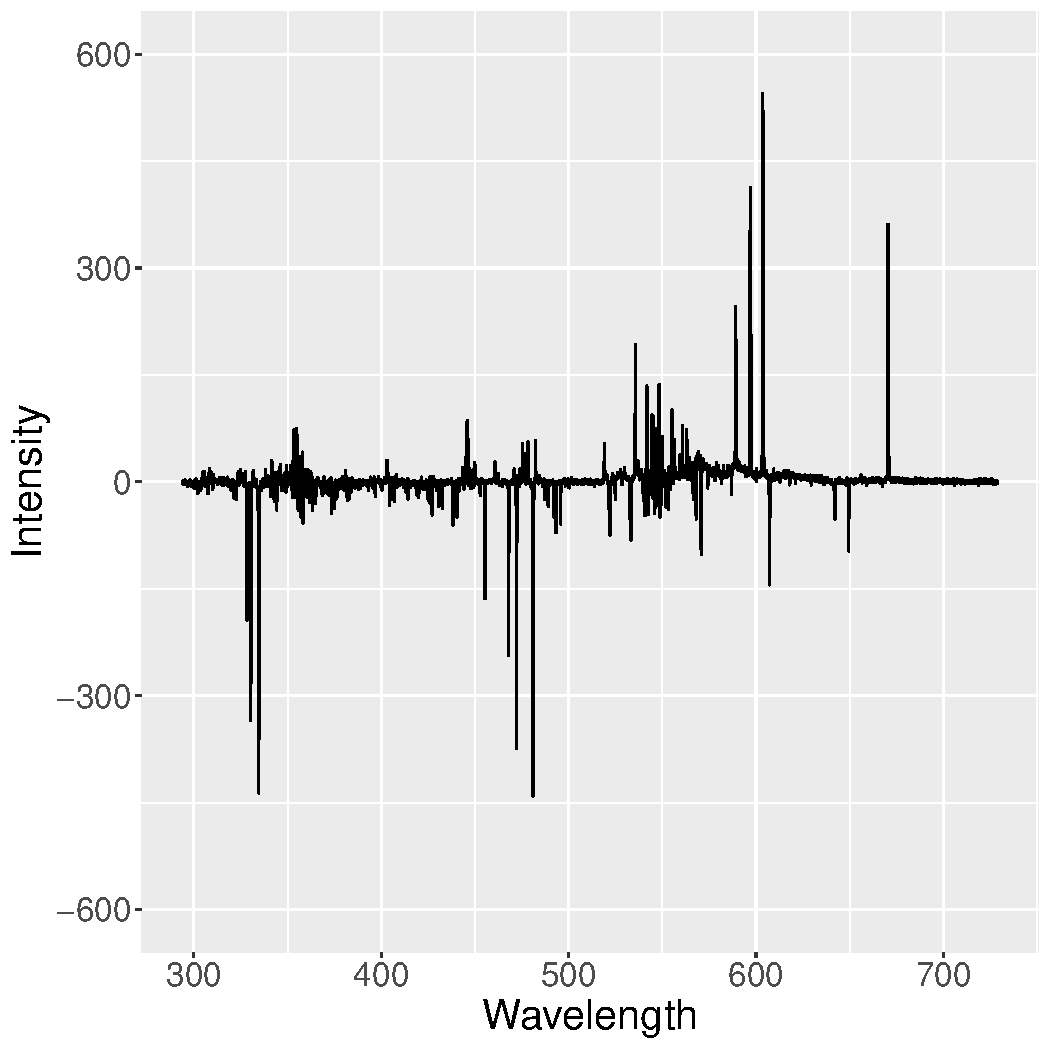
\includegraphics[width=\textwidth]{M14_04.pdf}
    \end{subfigure}
    \caption{\textbf{Gráficos para análisis de outliers}.}  
    \label{fig:outlier_analysis}
\end{figure}

\newpage
\section*{Anexo B: Algoritmo de LDA}
\addcontentsline{toc}{section}{Anexo B: Algoritmo de LDA}

Para la matriz de datos $\mathbf{X}$ con $N$ observaciones y $P$ variables, se estima tanto la matriz covarianza $\hat{\boldsymbol{\Sigma}}$ como la matriz covarianza de las medias de las clases $\hat{\boldsymbol{\Sigma}}_B$:

\begin{equation} \label{eq:cov}
\hat{\boldsymbol{\Sigma}} = \frac{1}{N-N_g} (\mathbf{X} - \mathbf{GM})^T (\mathbf{X} - \mathbf{GM}); \text{  }
\hat{\boldsymbol{\Sigma}}_B = \frac{N \boldsymbol{\pi}}{N_g - 1} (\mathbf{GM} - \mathbf{1}\boldsymbol{\mu})^T (\mathbf{GM} - \mathbf{1}\boldsymbol{\mu})
\end{equation}

donde $GM$ es una matriz cuyas filas son vectores de media $\boldsymbol{\mu}_j$ correspondientes a cada observación de $X$ y $N_g$ es número de grupos, $\boldsymbol{\pi}$ es un vector de probabilidades a priori de cada grupo, $\mathbf{1}$ es un vector de unos de $N$X$1$ y $\boldsymbol{\mu}$ es una media ponderada: $\boldsymbol{\mu} = \Sigma_j \boldsymbol{\pi}_j \boldsymbol{\mu}_j$.
%\begin{equation} \label{eq:covb}
%\hat{\boldsymbol{\Sigma}}_B = \frac{N \boldsymbol{\pi}}{N_g - 1} (\mathbf{GM} - \mathbf{1}\boldsymbol{\mu})^T (\mathbf{GM} - \mathbf{1}\boldsymbol{\mu})
%\end{equation}
%donde $\boldsymbol{\pi}$ es un vector conteniendo las probabilidades a priori de cada grupo y $\boldsymbol{\mu}$ es la media ponderada de las medias de grupo: $\boldsymbol{\mu} = \Sigma_j \boldsymbol{\pi}_j \boldsymbol{\mu}_j$.

Se busca una transformación que separe los grupos lo más posible (esto se hace maximizando la dispersión entre clases, $bss$) mientras que al mismo tiempo minimice la dispersión dentro de cada grupo ($wss$), para ello, se busca una dirección representada por el vector unitario $\mathbf{v}_b$ tal que la proyección de los datos cumpla con:

\begin{equation} \label{eq:maxratio}
\max\{\frac{bss}{wss}\} = \max\{\frac{\mathbf{v}_b^T \hat{\boldsymbol{\Sigma}}_B \mathbf{v}_b}{\mathbf{v}_b^T \hat{\boldsymbol{\Sigma}} \mathbf{v}_b}\}
\end{equation}

Una vez que se obtiene $\mathbf{v}_b$, se repite varias veces el procedimiento sobre el subespacio ortogonal al vector (o vectores) obtenidos. Las variables obtenidas de esta forma son conocidas como \textit{variables canónicas o discriminantes}.

Para poder resolver este problema, primero se realiza una transformación esférica o blanqueamiento de los datos centrados. Esto es, con $\mathbf{X}_C = \mathbf{X} - \mathbf{1}\boldsymbol{\mu}$ y $\hat{\boldsymbol{\Sigma}} = \mathbf{V} \boldsymbol{\Lambda} \mathbf{V}^T$, se calcula $\mathbf{X}_C \mathbf{V} \boldsymbol{\Lambda}^{-\frac{1}{2}}$, lo que hace que $\hat{\boldsymbol{\Sigma}} = \mathbf{I}_P$ en el nuevo espacio y luego se buscan las direcciones que maximicen $bss$ (esto es, los autovectores de $\hat{\boldsymbol{\Sigma}}_B$). Como consecuencia esta restricción, las direcciones deseadas (en el espacio original) se calculan mediante los autovectores de $\hat{\boldsymbol{\Sigma}}^{-1}\hat{\boldsymbol{\Sigma}}_B$.

%\textit{La supresión de dimensiones problemáticas correspondientes al ruido se hace en este paso.} Si se toma la autodescomposición de la Ecuación \ref{eq:eigendecomposition} y se suprimen las dimensiones con ruido ($\lambda_p < tol$), se obtendrá una matriz reconstruida:

%\begin{equation} \label{eq:reduction}
%\hat{\Sigma'}^{-1} = (V' \Lambda' V'^T)^{-1} = \sum_{p = 1}^{A} v_p (\frac{1}{\lambda_p}) v_p^T 
%\end{equation}

La implementación de \textit{lda} de la librería \textit{MASS} se aprovecha la descomposición en valores únicos (SVD) la cual tiene una implementación eficiente en la librería \textit{LAPACK} y evita el cálculo explícito de matrices inversas (o el armado de las matrices covarianza): 

\begin{enumerate}
    \item Se escala cada variable utilizando sus medianas estándar $\sigma(\mathbf{X} - \mathbf{GM})$.
    \item Se calcula $\mathbf{M} = \frac{1}{\sqrt{N - N_g}} (\mathbf{X} - \mathbf{GM})$, de manera que $\hat{\boldsymbol{\Sigma}} = \mathbf{M}^T \mathbf{M}$.
    \item Se calcula el SVD de $\mathbf{M}$: $\mathbf{M} = \mathbf{U} \mathbf{S} \mathbf{V}^T$, de manera que $\hat{\boldsymbol{\Sigma}}^{-1} = \mathbf{V} \mathbf{S}^{-2} \mathbf{V}^T$.
    \item Se centran los datos (y las medias) respecto de la media ponderada $\boldsymbol{\mu}$.
    \item Se aplica una transformación esférica o blanqueamiento sobre los datos (y las medias): 
    $\mathbf{X}_S = \mathbf{X}_C \mathbf{V}' \mathbf{S}'^{-1}$. Nótese que se suprimen las dimensiones $P' + 1$ a $P$ para las cuales $s_{pp} < tol$ ($\mathbf{V}' = \mathbf{V}[1,\ldots,P;1,\ldots,P']$ y $\mathbf{S} = \mathbf{S}[1,\ldots,P';1,\ldots,P']$)
    \item Se calcula $\mathbf{M}_B = \sqrt{\frac{N \boldsymbol{\pi}}{N_g - 1}} \odot  (\mathbf{GM}_S - \mathbf{1}\boldsymbol{\mu}_S)$, de manera que en el espacio esferizado $\hat{\boldsymbol{\Sigma}}_{BS} = \mathbf{M}_B^T \mathbf{M}_B$
    \item Se realiza la descomposición en valores únicos de $\mathbf{M}_B$: $\mathbf{M}_B = \mathbf{U}_B \mathbf{S}_B \mathbf{V}_B^T$. Se suprimen las dimensiones tales que $s_{Bpp} < tol s_{B00}$.
    \item Se transforman los datos (y las medias) a una nueva base de manera de maximizar la separación entre grupos: $\mathbf{X}^* = \mathbf{X}_S \mathbf{V}'_B$, de manera que la transformación final resulta: $\mathbf{X}^* = \mathbf{X}_C \mathbf{V}' \mathbf{S}'^{-1} \mathbf{V}'_B$.
    \item Finalmente se calculan las funciones discriminantes: $\mathbf{X}^* {\mathbf{GM}^*}^T - \frac{1}{2} \mathbf{GM}^* {\mathbf{GM}^*}^T + \mathbf{1} \log \boldsymbol{\pi} $
\end{enumerate}

\end{document}
